\hypertarget{ux446ux435ux43bux44c-ux440ux430ux431ux43eux442ux44b}{%
\section{Цель
работы}\label{ux446ux435ux43bux44c-ux440ux430ux431ux43eux442ux44b}}

Ознакомиться с функционалом операционной системы Linux.

\hypertarget{ux437ux430ux434ux430ux43dux438ux435}{%
\section{Задание}\label{ux437ux430ux434ux430ux43dux438ux435}}

Просмотреть видео и на основе полученной информации пройти тестовые
задания.

\hypertarget{ux432ux44bux43fux43eux43bux43dux435ux43dux438ux435-ux43bux430ux431ux43eux440ux430ux442ux43eux440ux43dux43eux439-ux440ux430ux431ux43eux442ux44b}{%
\section{Выполнение лабораторной
работы}\label{ux432ux44bux43fux43eux43bux43dux435ux43dux438ux435-ux43bux430ux431ux43eux440ux430ux442ux43eux440ux43dux43eux439-ux440ux430ux431ux43eux442ux44b}}

1 Этап:

\begin{figure}
\hypertarget{fig:001}{%
\centering
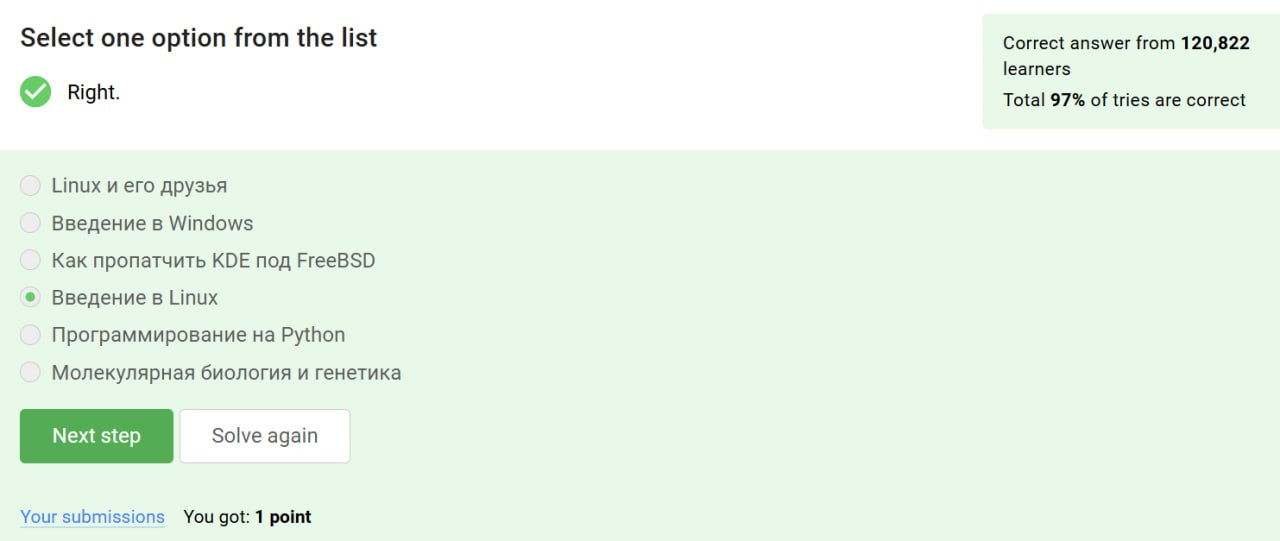
\includegraphics[width=0.7\textwidth,height=\textheight]{image/1.png}
\caption{1}\label{fig:001}
}
\end{figure}

\hypertarget{ux432ux44bux43fux43eux43bux43dux435ux43dux438ux435-ux43bux430ux431ux43eux440ux430ux442ux43eux440ux43dux43eux439-ux440ux430ux431ux43eux442ux44b-1}{%
\section{Выполнение лабораторной
работы}\label{ux432ux44bux43fux43eux43bux43dux435ux43dux438ux435-ux43bux430ux431ux43eux440ux430ux442ux43eux440ux43dux43eux439-ux440ux430ux431ux43eux442ux44b-1}}

Курс действительно называется ``Введение в Linux'', поэтому с этим
вопросом проблем не возникло.

\begin{figure}
\hypertarget{fig:002}{%
\centering
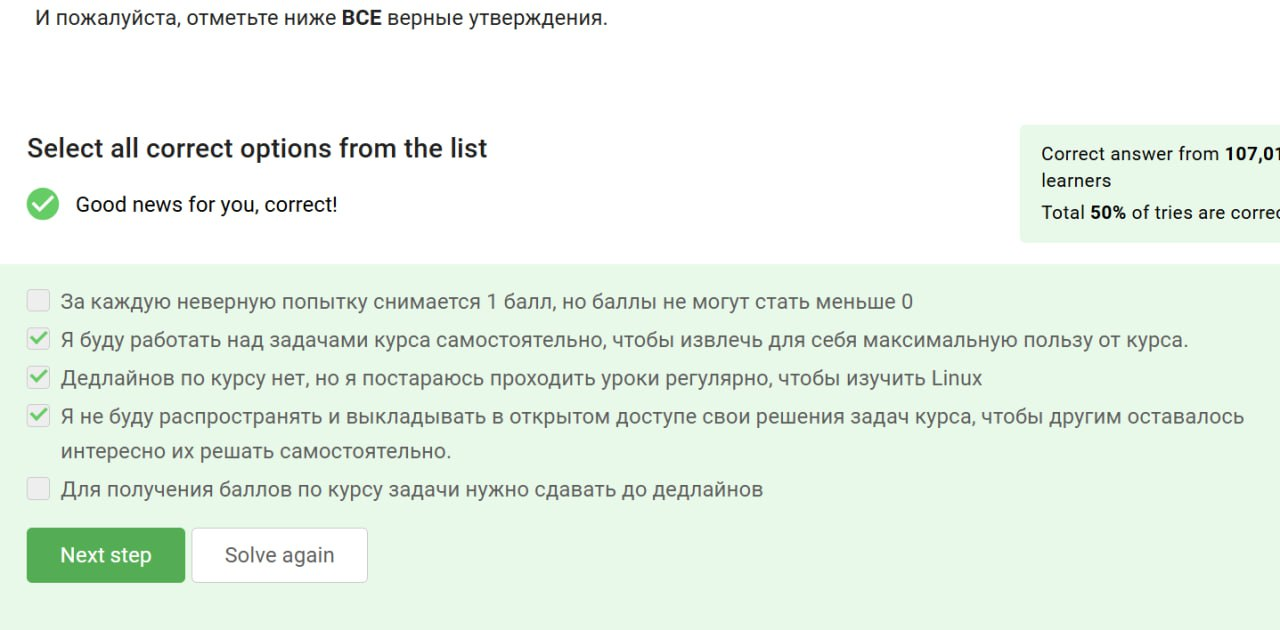
\includegraphics[width=0.7\textwidth,height=\textheight]{image/2.png}
\caption{2}\label{fig:002}
}
\end{figure}

\hypertarget{ux432ux44bux43fux43eux43bux43dux435ux43dux438ux435-ux43bux430ux431ux43eux440ux430ux442ux43eux440ux43dux43eux439-ux440ux430ux431ux43eux442ux44b-2}{%
\section{Выполнение лабораторной
работы}\label{ux432ux44bux43fux43eux43bux43dux435ux43dux438ux435-ux43bux430ux431ux43eux440ux430ux442ux43eux440ux43dux43eux439-ux440ux430ux431ux43eux442ux44b-2}}

Прочитав критерии прохождения курса, я отметила необходимые утверждения.

\begin{figure}
\hypertarget{fig:003}{%
\centering
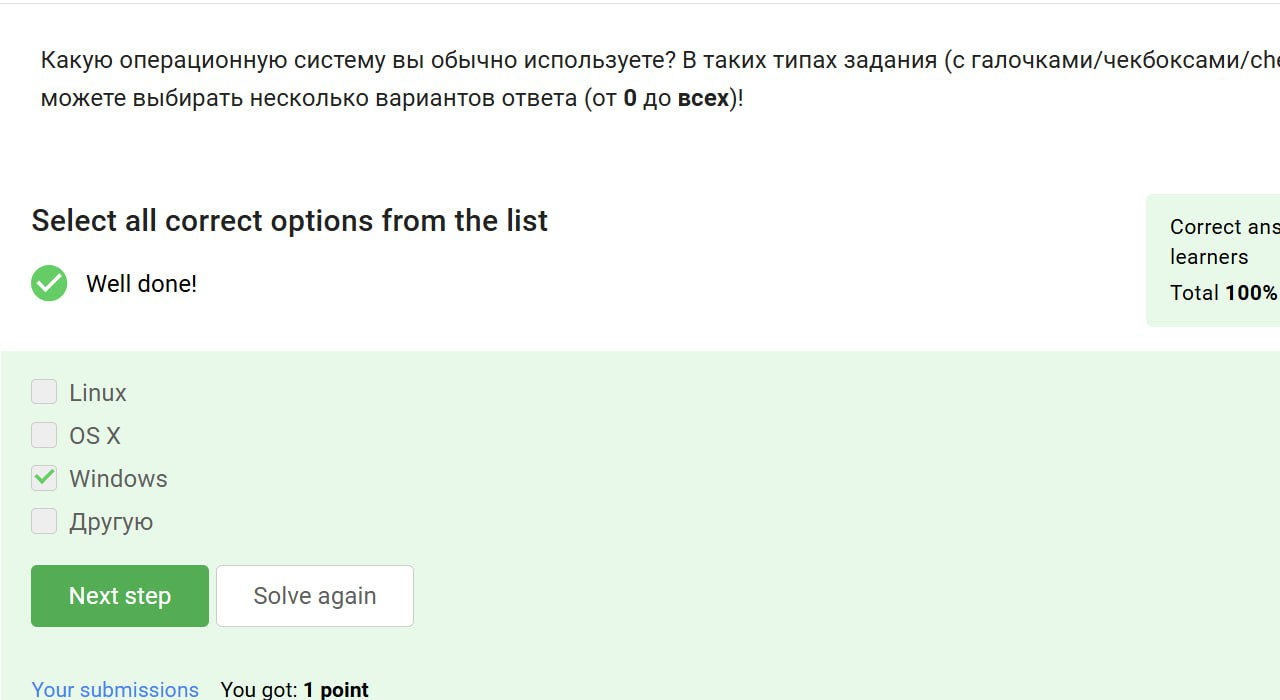
\includegraphics[width=0.7\textwidth,height=\textheight]{image/3.png}
\caption{3}\label{fig:003}
}
\end{figure}

\hypertarget{ux432ux44bux43fux43eux43bux43dux435ux43dux438ux435-ux43bux430ux431ux43eux440ux430ux442ux43eux440ux43dux43eux439-ux440ux430ux431ux43eux442ux44b-3}{%
\section{Выполнение лабораторной
работы}\label{ux432ux44bux43fux43eux43bux43dux435ux43dux438ux435-ux43bux430ux431ux43eux440ux430ux442ux43eux440ux43dux43eux439-ux440ux430ux431ux43eux442ux44b-3}}

Стандартная операционная система, предлагаемая большей частью магазинов
- windows, именно она стоит у меня на основном компьютере.

\begin{figure}
\hypertarget{fig:004}{%
\centering
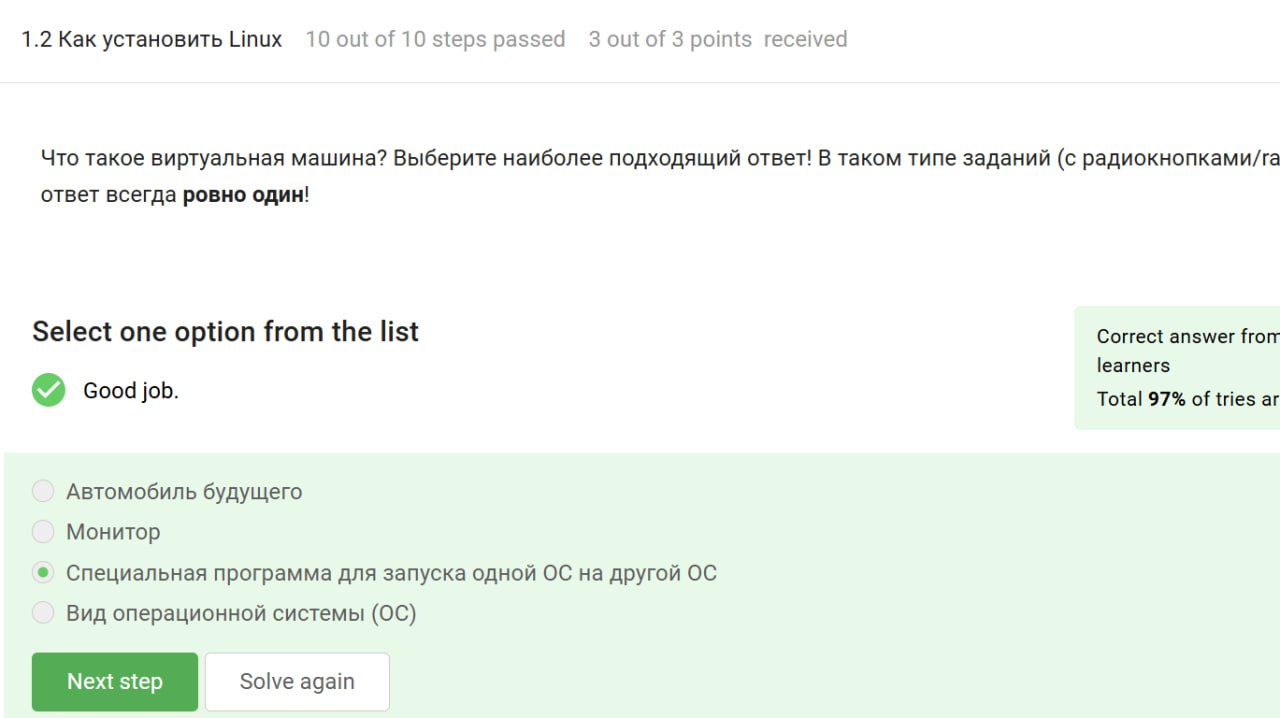
\includegraphics[width=0.7\textwidth,height=\textheight]{image/4.png}
\caption{4}\label{fig:004}
}
\end{figure}

\hypertarget{ux432ux44bux43fux43eux43bux43dux435ux43dux438ux435-ux43bux430ux431ux43eux440ux430ux442ux43eux440ux43dux43eux439-ux440ux430ux431ux43eux442ux44b-4}{%
\section{Выполнение лабораторной
работы}\label{ux432ux44bux43fux43eux43bux43dux435ux43dux438ux435-ux43bux430ux431ux43eux440ux430ux442ux43eux440ux43dux43eux439-ux440ux430ux431ux43eux442ux44b-4}}

На свой компьютер мы устанавливали специальную программу VirtualBox,
которая нужна для подключения одной операционной на другой.

\begin{figure}
\hypertarget{fig:005}{%
\centering
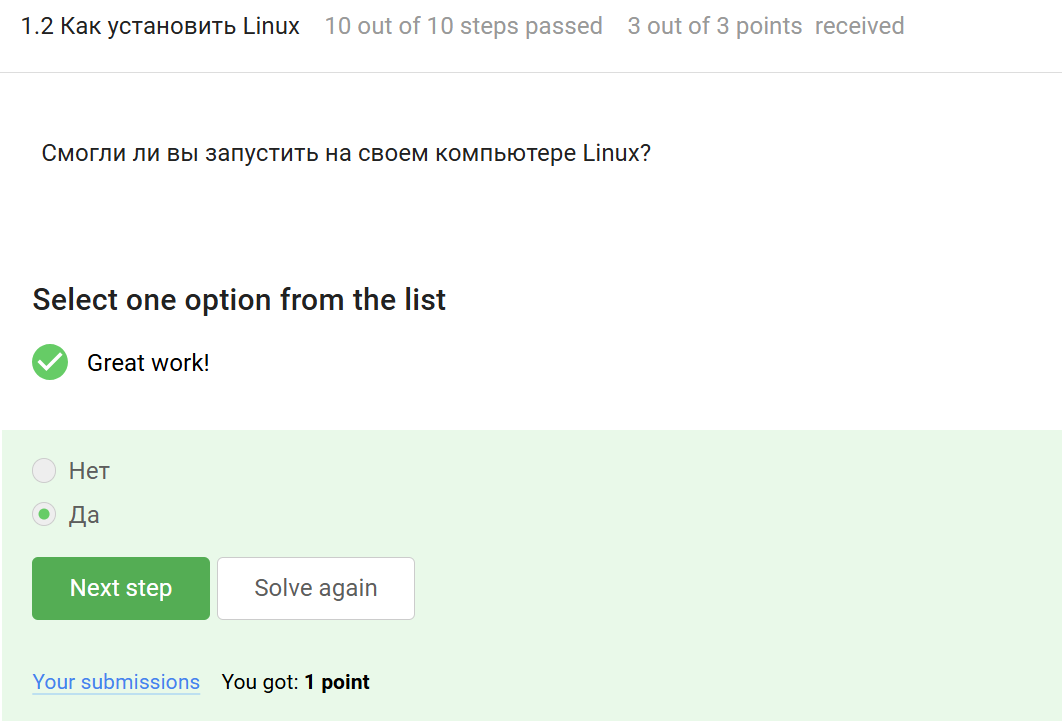
\includegraphics[width=0.7\textwidth,height=\textheight]{image/5.png}
\caption{5}\label{fig:005}
}
\end{figure}

\hypertarget{ux432ux44bux43fux43eux43bux43dux435ux43dux438ux435-ux43bux430ux431ux43eux440ux430ux442ux43eux440ux43dux43eux439-ux440ux430ux431ux43eux442ux44b-5}{%
\section{Выполнение лабораторной
работы}\label{ux432ux44bux43fux43eux43bux43dux435ux43dux438ux435-ux43bux430ux431ux43eux440ux430ux442ux43eux440ux43dux43eux439-ux440ux430ux431ux43eux442ux44b-5}}

Да, моя виртуальная машина хорошо работает, и у меня получилось
запустить с неё Линукс

\begin{figure}
\hypertarget{fig:006}{%
\centering
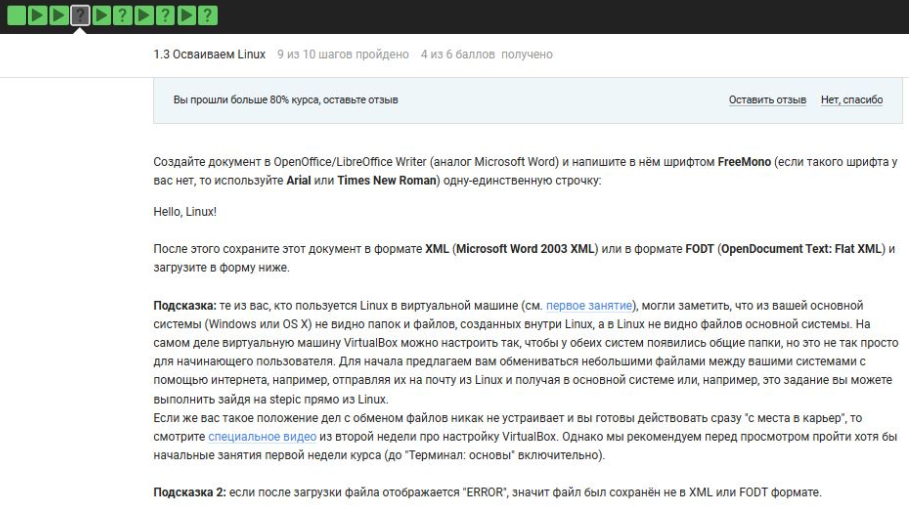
\includegraphics[width=0.7\textwidth,height=\textheight]{image/6.png}
\caption{6}\label{fig:006}
}
\end{figure}

Я создала документ, и перед сохранением выбрала нужный формат, а после я
ег прикрепила к курсу. Прикрепленный файл видно на скриншоте.

\begin{figure}
\hypertarget{fig:007}{%
\centering
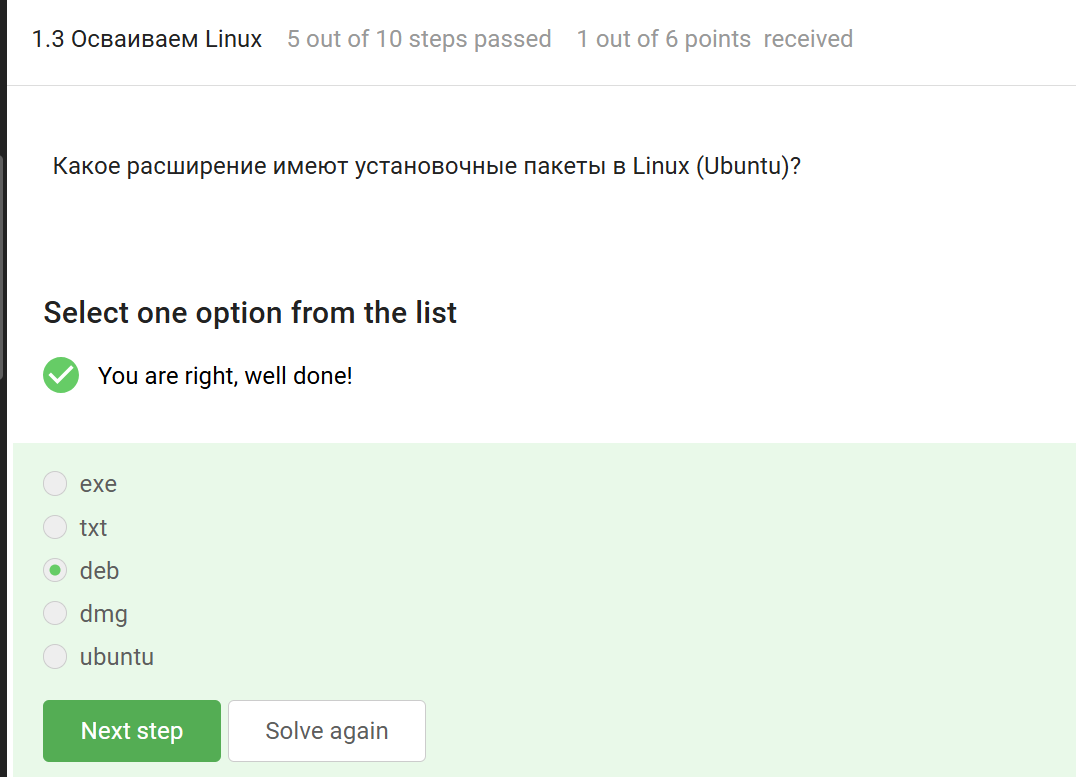
\includegraphics[width=0.7\textwidth,height=\textheight]{image/7.png}
\caption{7}\label{fig:007}
}
\end{figure}

\hypertarget{ux432ux44bux43fux43eux43bux43dux435ux43dux438ux435-ux43bux430ux431ux43eux440ux430ux442ux43eux440ux43dux43eux439-ux440ux430ux431ux43eux442ux44b-6}{%
\section{Выполнение лабораторной
работы}\label{ux432ux44bux43fux43eux43bux43dux435ux43dux438ux435-ux43bux430ux431ux43eux440ux430ux442ux43eux440ux43dux43eux439-ux440ux430ux431ux43eux442ux44b-6}}

deb --- формат пакетов операционных систем проекта Debian. Используется
также их производными, такими как Ubuntu, Knoppix и другими.

\begin{figure}
\hypertarget{fig:008}{%
\centering
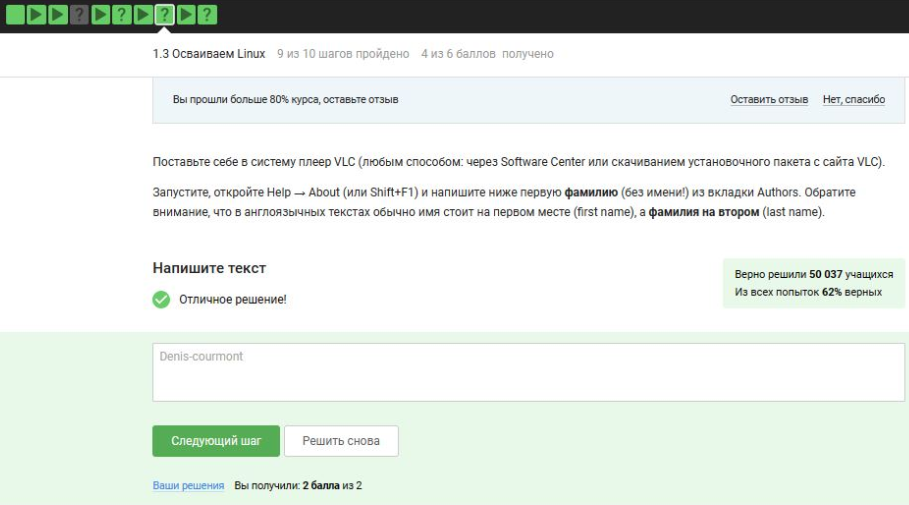
\includegraphics[width=0.7\textwidth,height=\textheight]{image/8.png}
\caption{8}\label{fig:008}
}
\end{figure}

\begin{figure}
\hypertarget{fig:009}{%
\centering
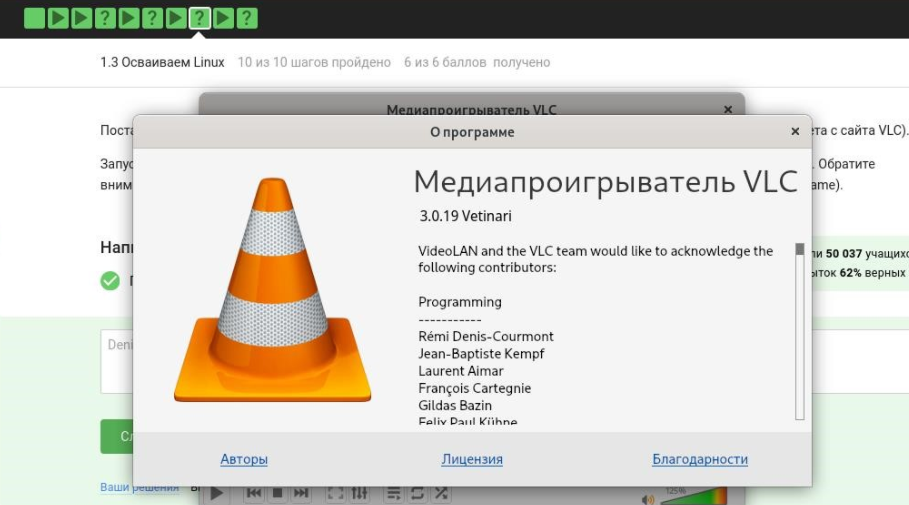
\includegraphics[width=0.7\textwidth,height=\textheight]{image/9.png}
\caption{9}\label{fig:009}
}
\end{figure}

\hypertarget{ux432ux44bux43fux43eux43bux43dux435ux43dux438ux435-ux43bux430ux431ux43eux440ux430ux442ux43eux440ux43dux43eux439-ux440ux430ux431ux43eux442ux44b-7}{%
\section{Выполнение лабораторной
работы}\label{ux432ux44bux43fux43eux43bux43dux435ux43dux438ux435-ux43bux430ux431ux43eux440ux430ux442ux43eux440ux43dux43eux439-ux440ux430ux431ux43eux442ux44b-7}}

Здесь на скриншоте видно, что установив программу медиапроигрывателя я
посмотрела, кто авторы программы и записала первую фамилию.

\begin{figure}
\hypertarget{fig:010}{%
\centering
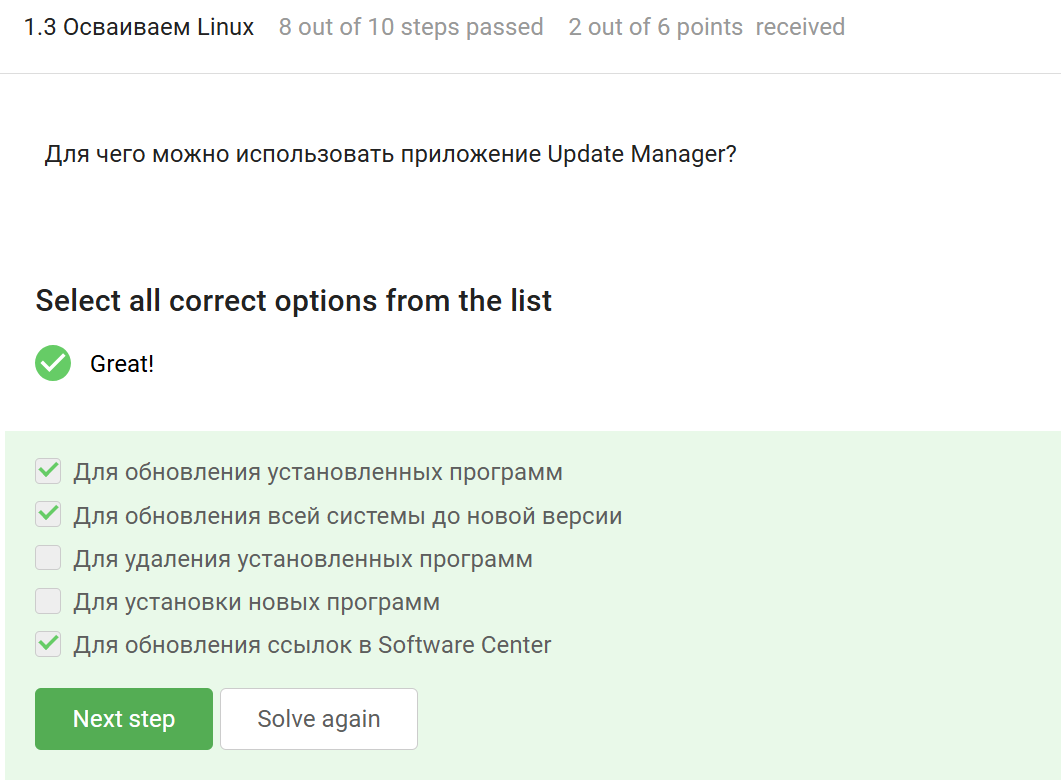
\includegraphics[width=0.7\textwidth,height=\textheight]{image/10.png}
\caption{10}\label{fig:010}
}
\end{figure}

\hypertarget{ux432ux44bux43fux43eux43bux43dux435ux43dux438ux435-ux43bux430ux431ux43eux440ux430ux442ux43eux440ux43dux43eux439-ux440ux430ux431ux43eux442ux44b-8}{%
\section{Выполнение лабораторной
работы}\label{ux432ux44bux43fux43eux43bux43dux435ux43dux438ux435-ux43bux430ux431ux43eux440ux430ux442ux43eux440ux43dux43eux439-ux440ux430ux431ux43eux442ux44b-8}}

Менеджер обновлений --- это программа для обновления установленного
программного обеспечения в дистрибутивах ОС Linux, основанных на Debian
или использующих систему управления пакетами APT.

\begin{figure}
\hypertarget{fig:011}{%
\centering
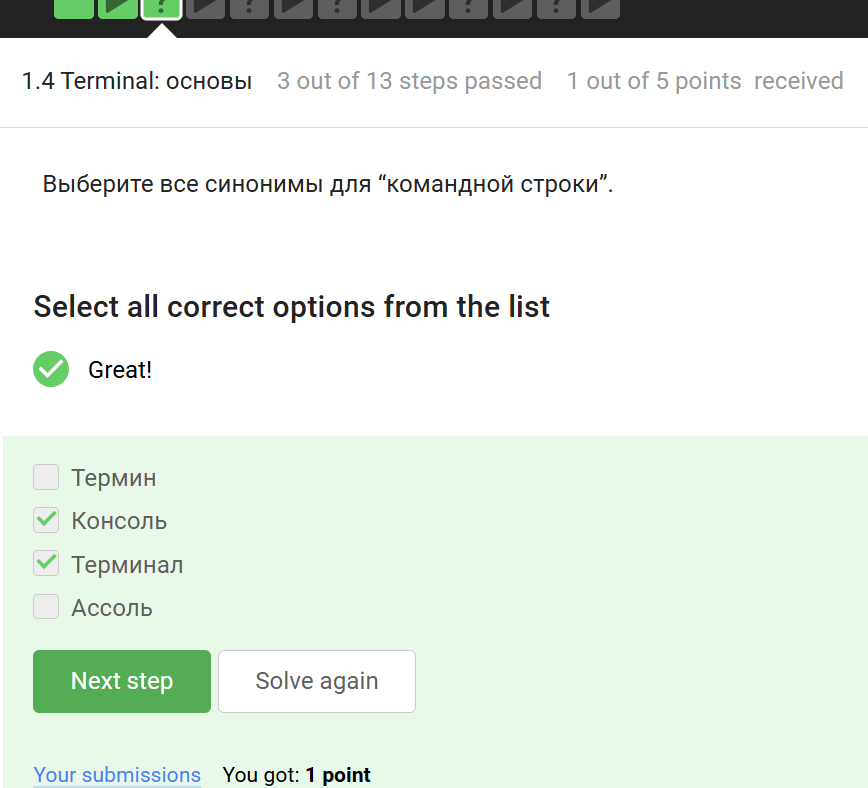
\includegraphics[width=0.7\textwidth,height=\textheight]{image/11.png}
\caption{11}\label{fig:011}
}
\end{figure}

Ассоль - героиня литературного произведения, а термин - это определение.

\begin{figure}
\hypertarget{fig:012}{%
\centering
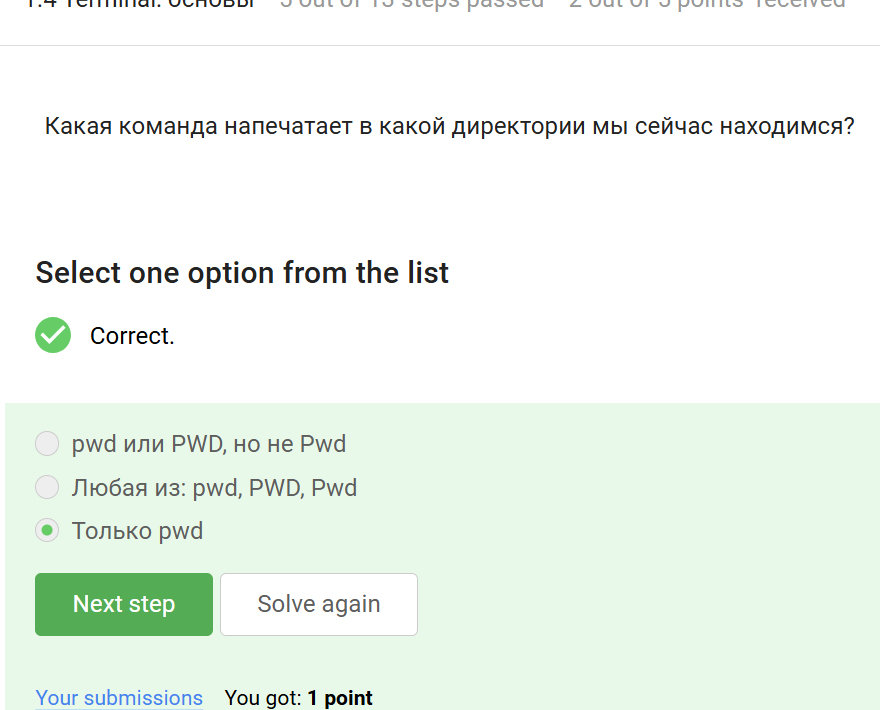
\includegraphics[width=0.7\textwidth,height=\textheight]{image/12.png}
\caption{12}\label{fig:012}
}
\end{figure}

\hypertarget{ux432ux44bux43fux43eux43bux43dux435ux43dux438ux435-ux43bux430ux431ux43eux440ux430ux442ux43eux440ux43dux43eux439-ux440ux430ux431ux43eux442ux44b-9}{%
\section{Выполнение лабораторной
работы}\label{ux432ux44bux43fux43eux43bux43dux435ux43dux438ux435-ux43bux430ux431ux43eux440ux430ux442ux43eux440ux43dux43eux439-ux440ux430ux431ux43eux442ux44b-9}}

Интерфейс командной строки Linux является регистрозависимым.

\begin{figure}
\hypertarget{fig:013}{%
\centering
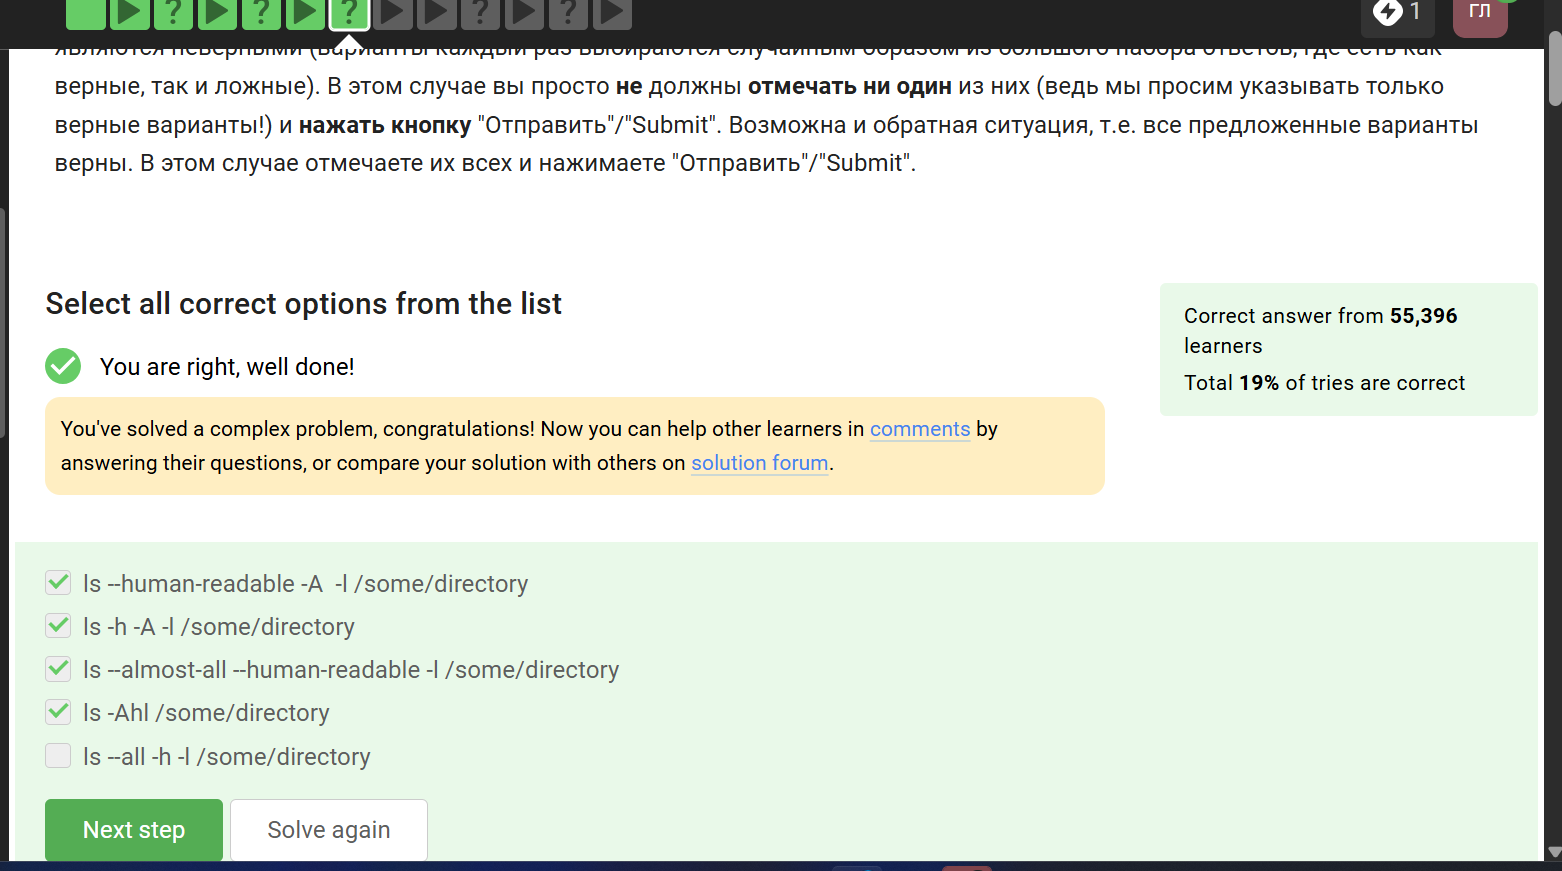
\includegraphics[width=0.7\textwidth,height=\textheight]{image/13.png}
\caption{13}\label{fig:013}
}
\end{figure}

\hypertarget{ux432ux44bux43fux43eux43bux43dux435ux43dux438ux435-ux43bux430ux431ux43eux440ux430ux442ux43eux440ux43dux43eux439-ux440ux430ux431ux43eux442ux44b-10}{%
\section{Выполнение лабораторной
работы}\label{ux432ux44bux43fux43eux43bux43dux435ux43dux438ux435-ux43bux430ux431ux43eux440ux430ux442ux43eux440ux43dux43eux439-ux440ux430ux431ux43eux442ux44b-10}}

Интерфейс командной строки Linux является регистрозависимым, поэтому не
подходит вариант, где буква А - маленькая(строчная).

\begin{figure}
\hypertarget{fig:014}{%
\centering
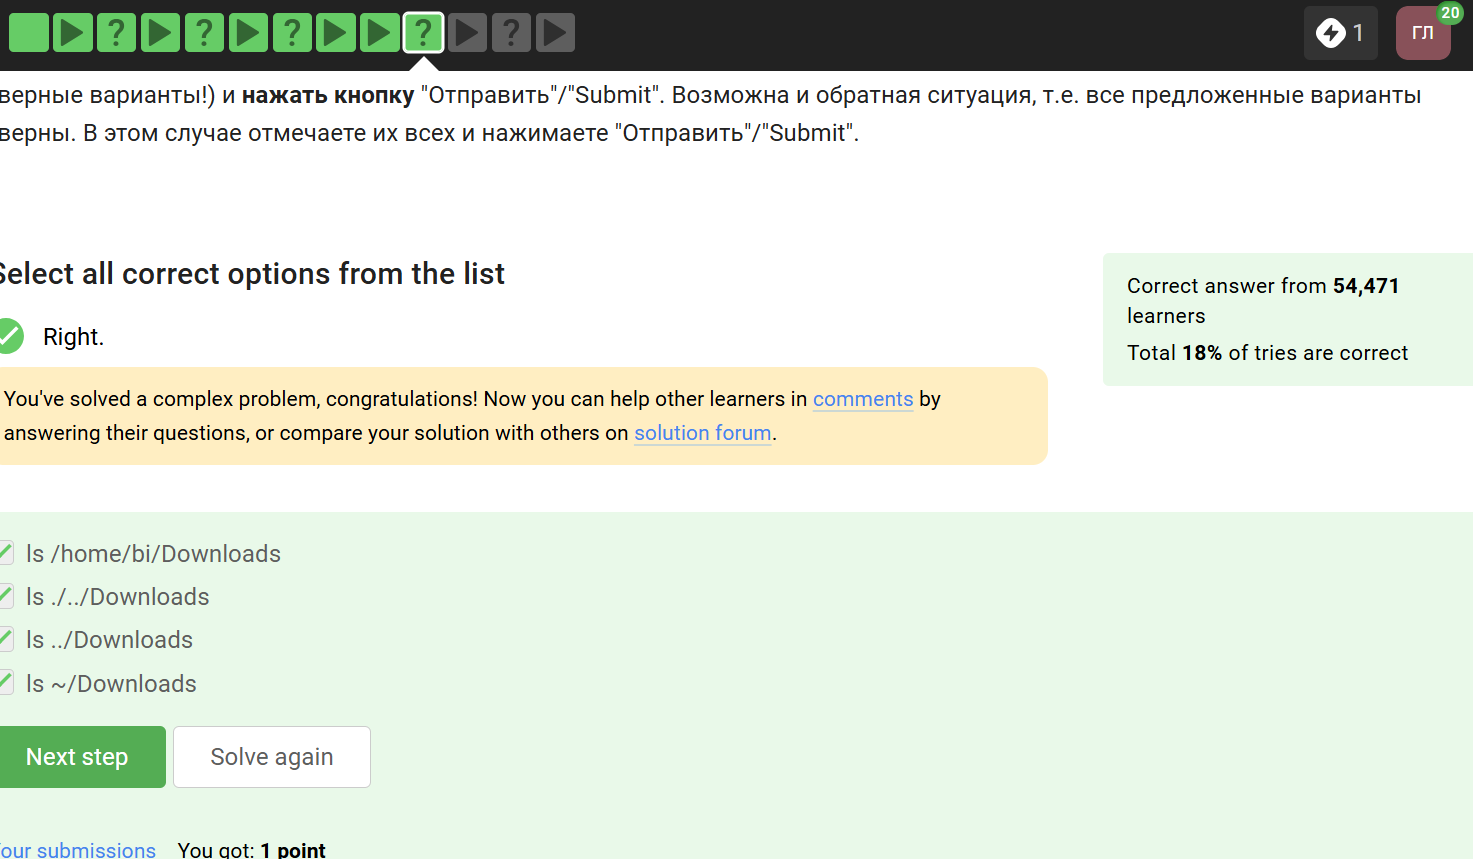
\includegraphics[width=0.7\textwidth,height=\textheight]{image/14.png}
\caption{14}\label{fig:014}
}
\end{figure}

Я прописываю полный путь до директории Downloads, так как на данный
момент нахожусь в другой директории.

\begin{figure}
\hypertarget{fig:015}{%
\centering
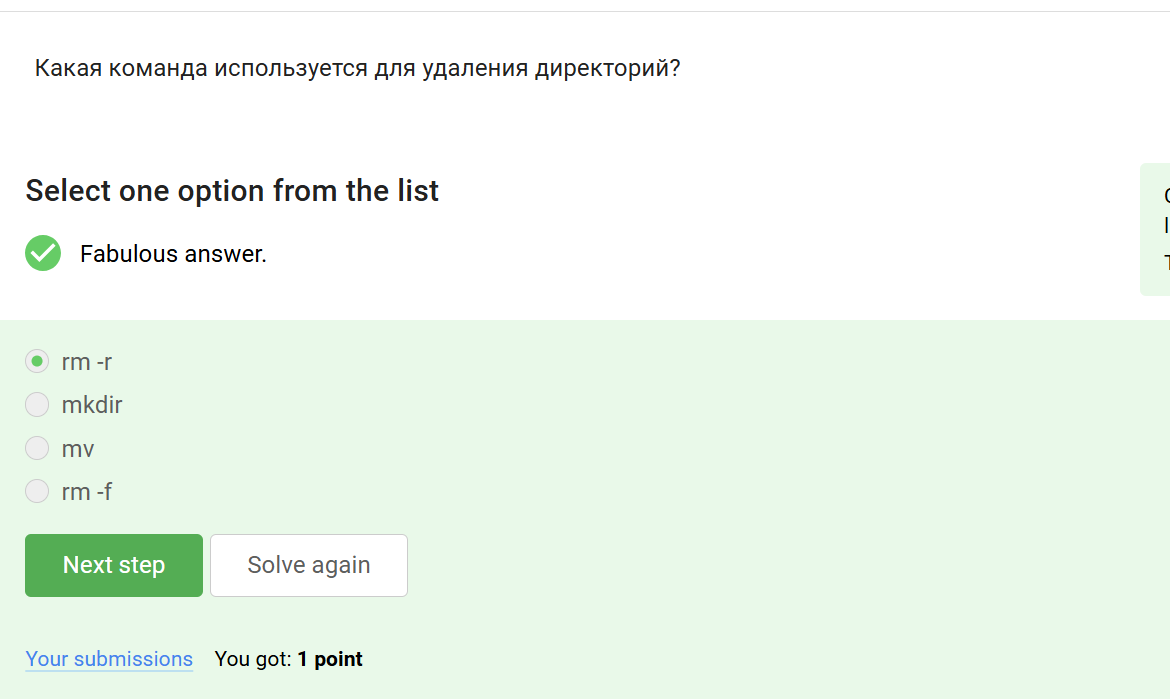
\includegraphics[width=0.7\textwidth,height=\textheight]{image/15.png}
\caption{15}\label{fig:015}
}
\end{figure}

\hypertarget{ux432ux44bux43fux43eux43bux43dux435ux43dux438ux435-ux43bux430ux431ux43eux440ux430ux442ux43eux440ux43dux43eux439-ux440ux430ux431ux43eux442ux44b-11}{%
\section{Выполнение лабораторной
работы}\label{ux432ux44bux43fux43eux43bux43dux435ux43dux438ux435-ux43bux430ux431ux43eux440ux430ux442ux43eux440ux43dux43eux439-ux440ux430ux431ux43eux442ux44b-11}}

rm -r удаление директории и рекуррентное удаление файлов, находящихся в
ней.

\begin{figure}
\hypertarget{fig:016}{%
\centering
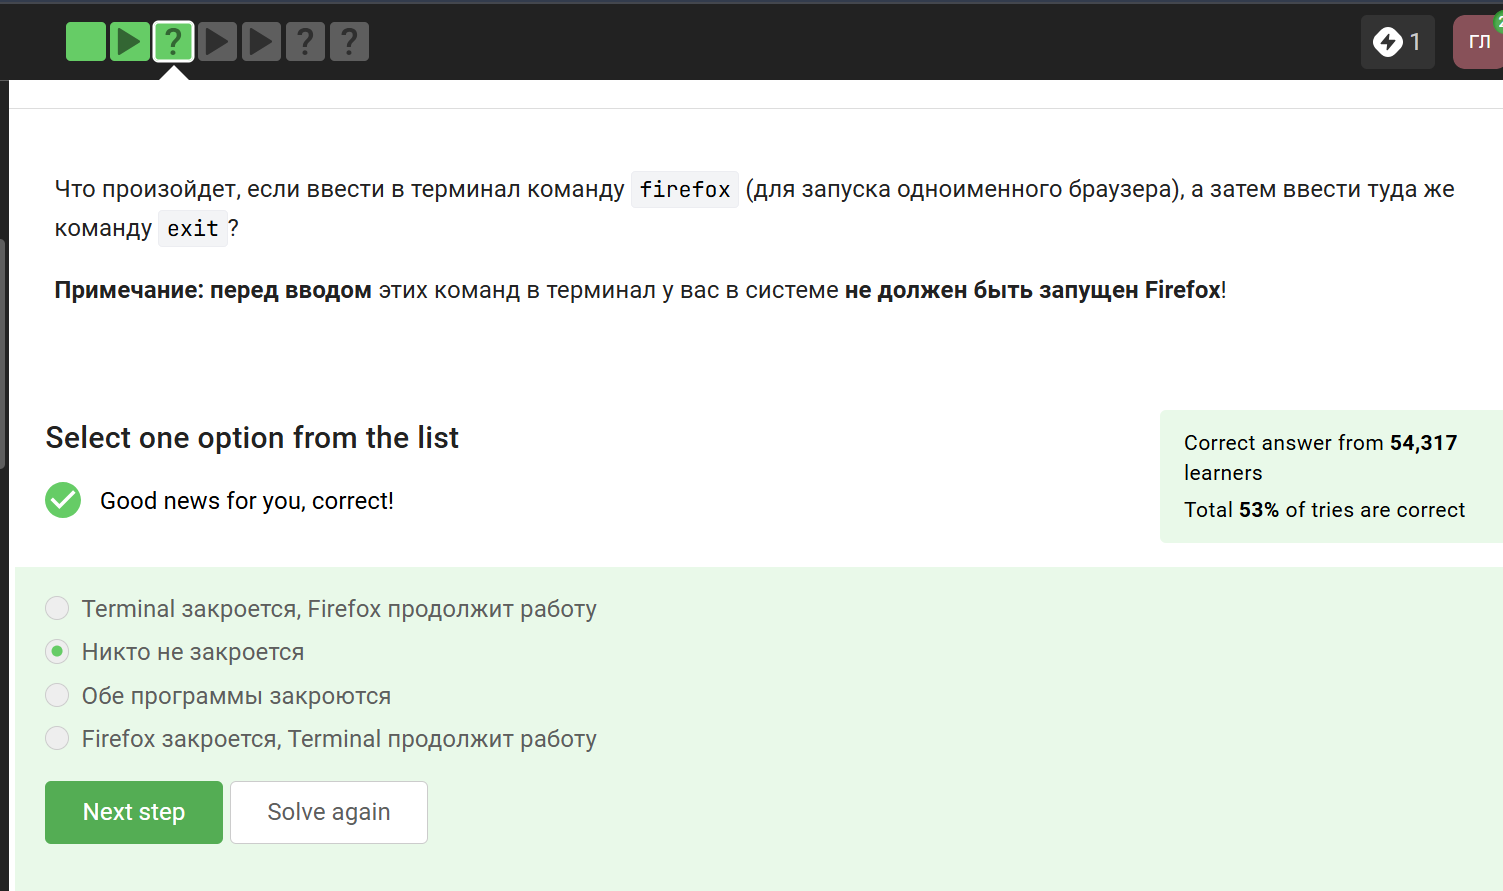
\includegraphics[width=0.7\textwidth,height=\textheight]{image/16.png}
\caption{16}\label{fig:016}
}
\end{figure}

\hypertarget{ux432ux44bux43fux43eux43bux43dux435ux43dux438ux435-ux43bux430ux431ux43eux440ux430ux442ux43eux440ux43dux43eux439-ux440ux430ux431ux43eux442ux44b-12}{%
\section{Выполнение лабораторной
работы}\label{ux432ux44bux43fux43eux43bux43dux435ux43dux438ux435-ux43bux430ux431ux43eux440ux430ux442ux43eux440ux43dux43eux439-ux440ux430ux431ux43eux442ux44b-12}}

Это я проверила эмпирическим путём, что видно в ходе скринкаста.

\begin{figure}
\hypertarget{fig:017}{%
\centering
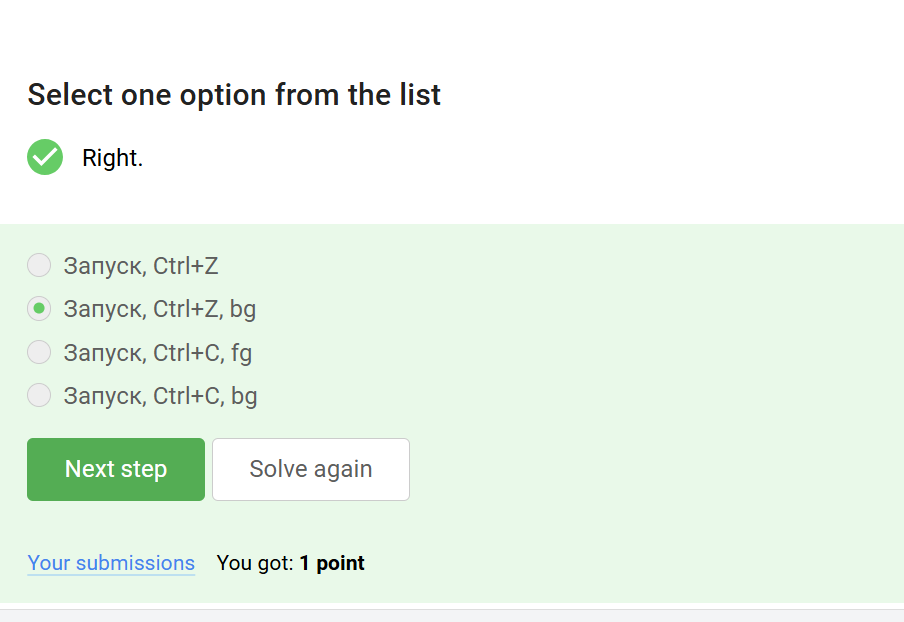
\includegraphics[width=0.7\textwidth,height=\textheight]{image/17.png}
\caption{17}\label{fig:017}
}
\end{figure}

\hypertarget{ux432ux44bux43fux43eux43bux43dux435ux43dux438ux435-ux43bux430ux431ux43eux440ux430ux442ux43eux440ux43dux43eux439-ux440ux430ux431ux43eux442ux44b-13}{%
\section{Выполнение лабораторной
работы}\label{ux432ux44bux43fux43eux43bux43dux435ux43dux438ux435-ux43bux430ux431ux43eux440ux430ux442ux43eux440ux43dux43eux439-ux440ux430ux431ux43eux442ux44b-13}}

Это запуск программы в фоновом режиме.

\begin{figure}
\hypertarget{fig:018}{%
\centering
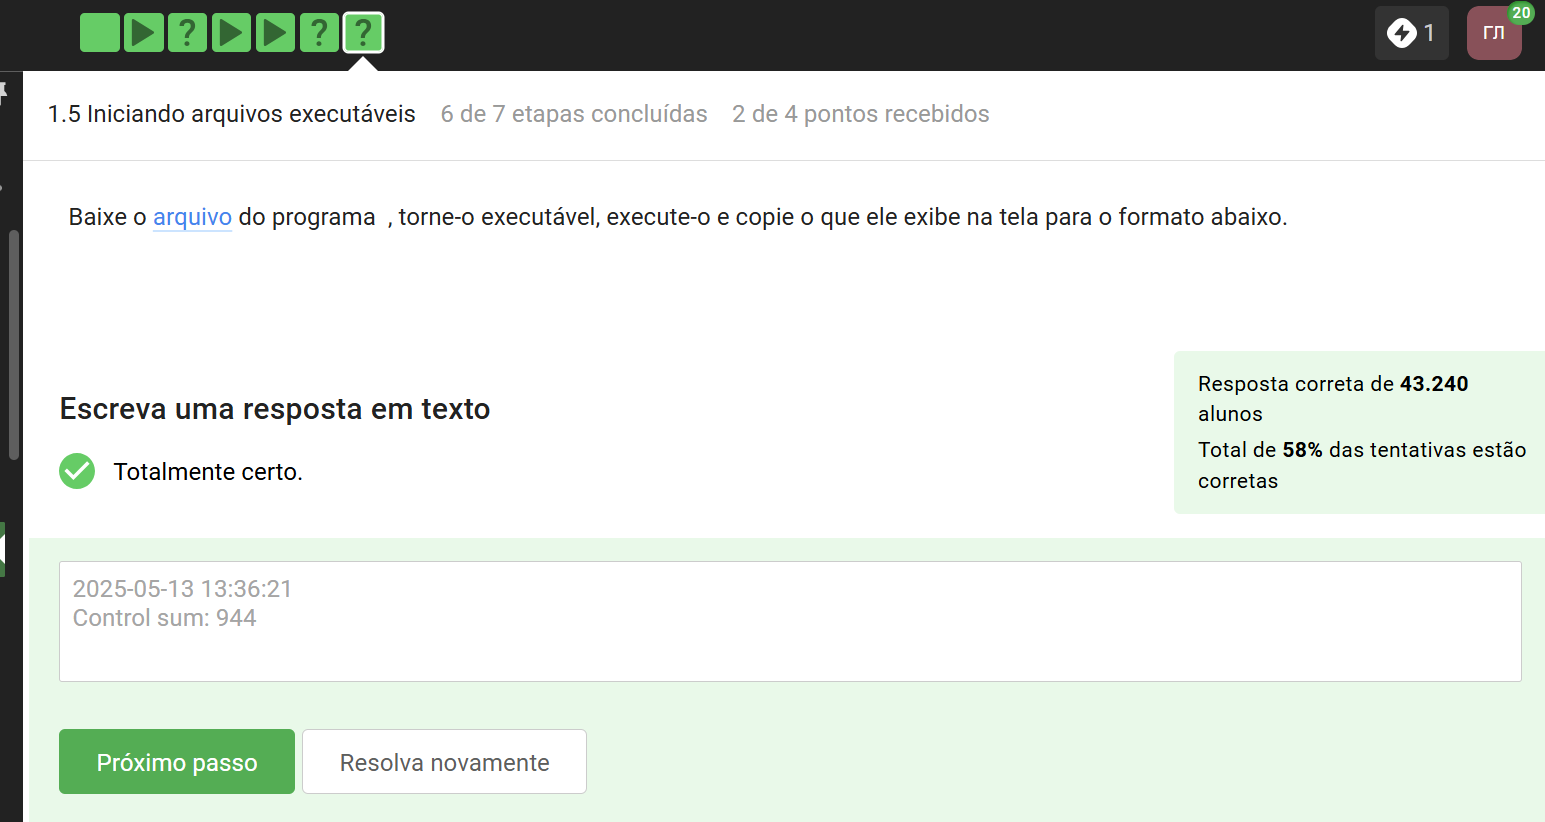
\includegraphics[width=0.7\textwidth,height=\textheight]{image/18.png}
\caption{18}\label{fig:018}
}
\end{figure}

\hypertarget{ux432ux44bux43fux43eux43bux43dux435ux43dux438ux435-ux43bux430ux431ux43eux440ux430ux442ux43eux440ux43dux43eux439-ux440ux430ux431ux43eux442ux44b-14}{%
\section{Выполнение лабораторной
работы}\label{ux432ux44bux43fux43eux43bux43dux435ux43dux438ux435-ux43bux430ux431ux43eux440ux430ux442ux43eux440ux43dux43eux439-ux440ux430ux431ux43eux442ux44b-14}}

Здесь видно выполнение команды.

\begin{figure}
\hypertarget{fig:020}{%
\centering
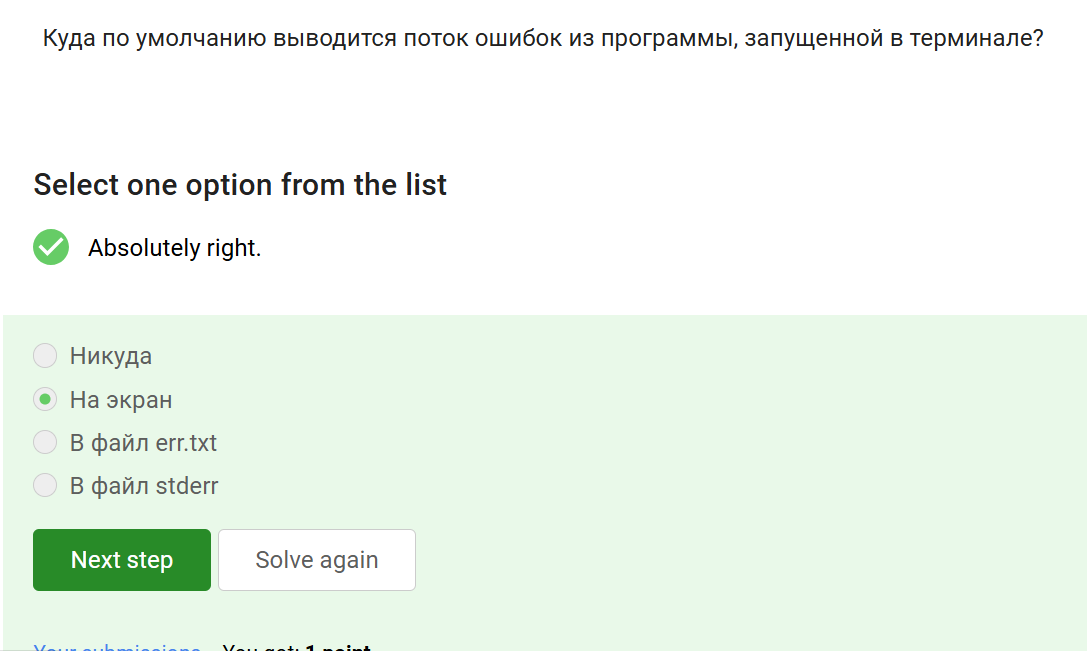
\includegraphics[width=0.7\textwidth,height=\textheight]{image/20.png}
\caption{20}\label{fig:020}
}
\end{figure}

Автоматически поток ошибок выводится на экран - это видно, например, в
ходе выполненных лабораторных. В файл будет поток выводиться, если его
перенаправить.

\begin{figure}
\hypertarget{fig:021}{%
\centering
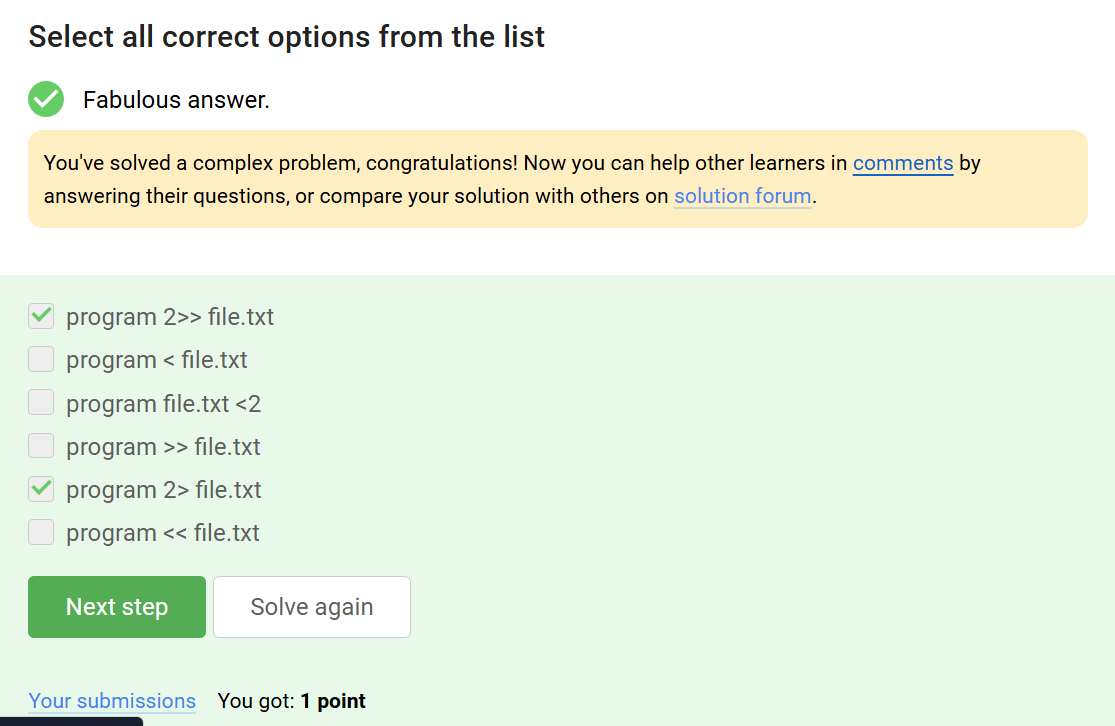
\includegraphics[width=0.7\textwidth,height=\textheight]{image/21.png}
\caption{21}\label{fig:021}
}
\end{figure}

\textless{} file --- использовать файл как источник данных для
стандартного потока ввода.

\hypertarget{ux432ux44bux43fux43eux43bux43dux435ux43dux438ux435-ux43bux430ux431ux43eux440ux430ux442ux43eux440ux43dux43eux439-ux440ux430ux431ux43eux442ux44b-15}{%
\section{Выполнение лабораторной
работы}\label{ux432ux44bux43fux43eux43bux43dux435ux43dux438ux435-ux43bux430ux431ux43eux440ux430ux442ux43eux440ux43dux43eux439-ux440ux430ux431ux43eux442ux44b-15}}

\begin{figure}
\hypertarget{fig:022}{%
\centering
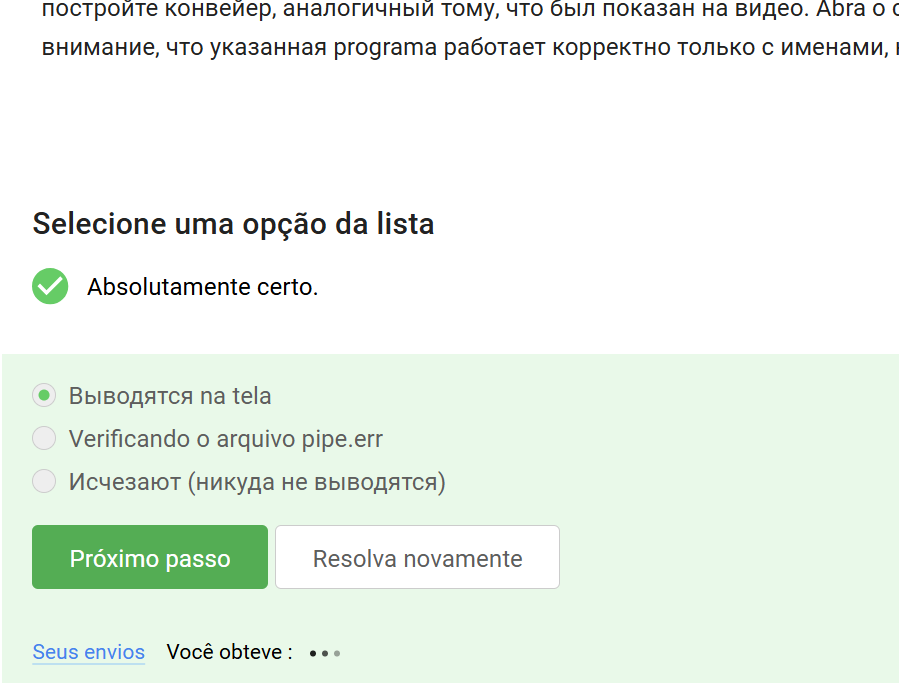
\includegraphics[width=0.7\textwidth,height=\textheight]{image/22.png}
\caption{22}\label{fig:022}
}
\end{figure}

\begin{enumerate}
\def\labelenumi{\arabic{enumi}.}
\item
  cat names.txt \textbar{} ./interacter.py \textbar{} less = вывод на
  экран
\item
  cat names.txt \textbar{} ./interacter.py 2\textgreater err.txt
  \textbar{} less = вывод ошибки в err.txt
\end{enumerate}

\begin{figure}
\hypertarget{fig:023}{%
\centering
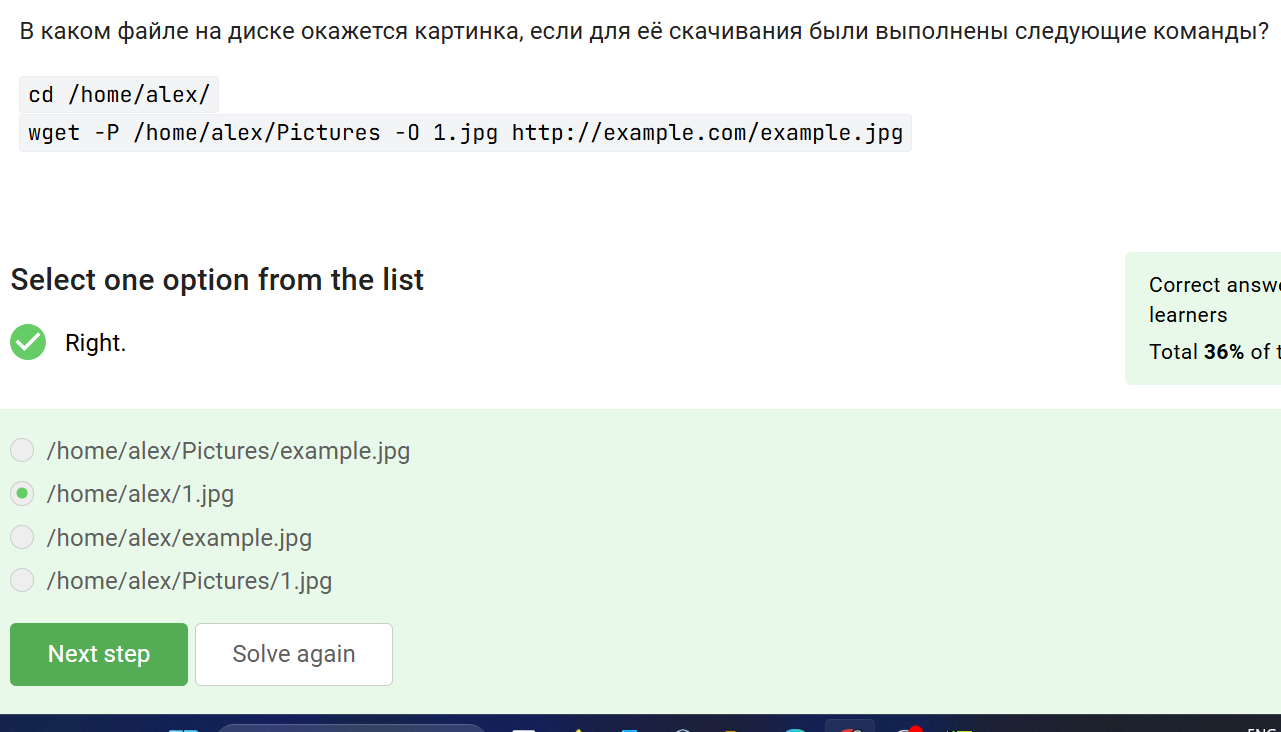
\includegraphics[width=0.7\textwidth,height=\textheight]{image/23.png}
\caption{23}\label{fig:023}
}
\end{figure}

\hypertarget{ux432ux44bux43fux43eux43bux43dux435ux43dux438ux435-ux43bux430ux431ux43eux440ux430ux442ux43eux440ux43dux43eux439-ux440ux430ux431ux43eux442ux44b-16}{%
\section{Выполнение лабораторной
работы}\label{ux432ux44bux43fux43eux43bux43dux435ux43dux438ux435-ux43bux430ux431ux43eux440ux430ux442ux43eux440ux43dux43eux439-ux440ux430ux431ux43eux442ux44b-16}}

Команда wget -P /home/alex/Pictures http://example.com/example.jpg
скачивает файл и даже размещает его, назвав example.jpg, в папке
/home/alex/Pictures.

\begin{figure}
\hypertarget{fig:024}{%
\centering
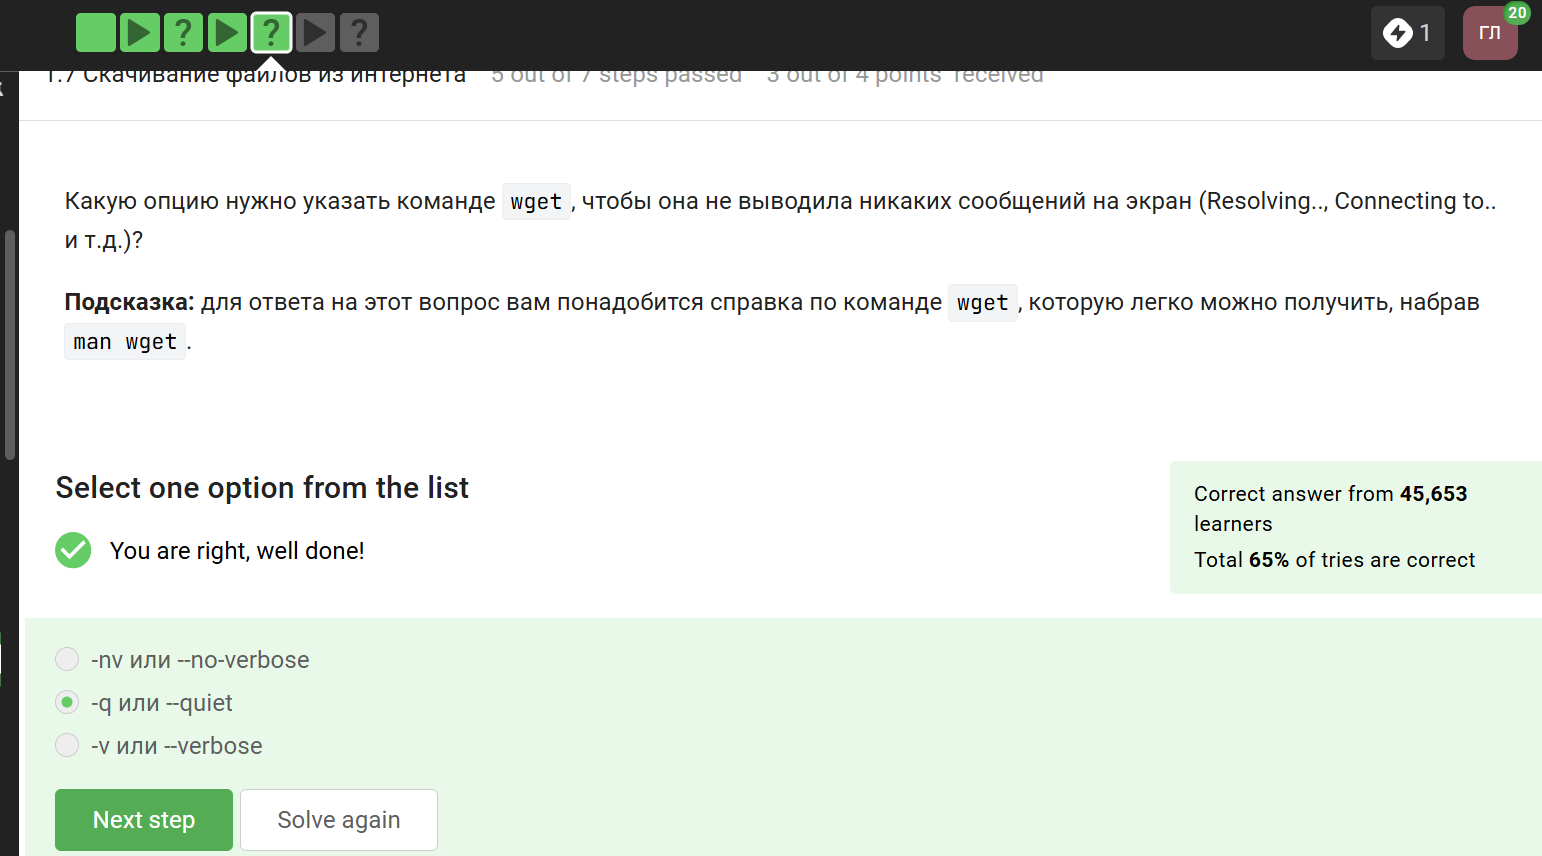
\includegraphics[width=0.7\textwidth,height=\textheight]{image/24.png}
\caption{24}\label{fig:024}
}
\end{figure}

-q --quiet Turn off Wget's output.

\hypertarget{ux432ux44bux43fux43eux43bux43dux435ux43dux438ux435-ux43bux430ux431ux43eux440ux430ux442ux43eux440ux43dux43eux439-ux440ux430ux431ux43eux442ux44b-17}{%
\section{Выполнение лабораторной
работы}\label{ux432ux44bux43fux43eux43bux43dux435ux43dux438ux435-ux43bux430ux431ux43eux440ux430ux442ux43eux440ux43dux43eux439-ux440ux430ux431ux43eux442ux44b-17}}

\begin{figure}
\hypertarget{fig:025}{%
\centering
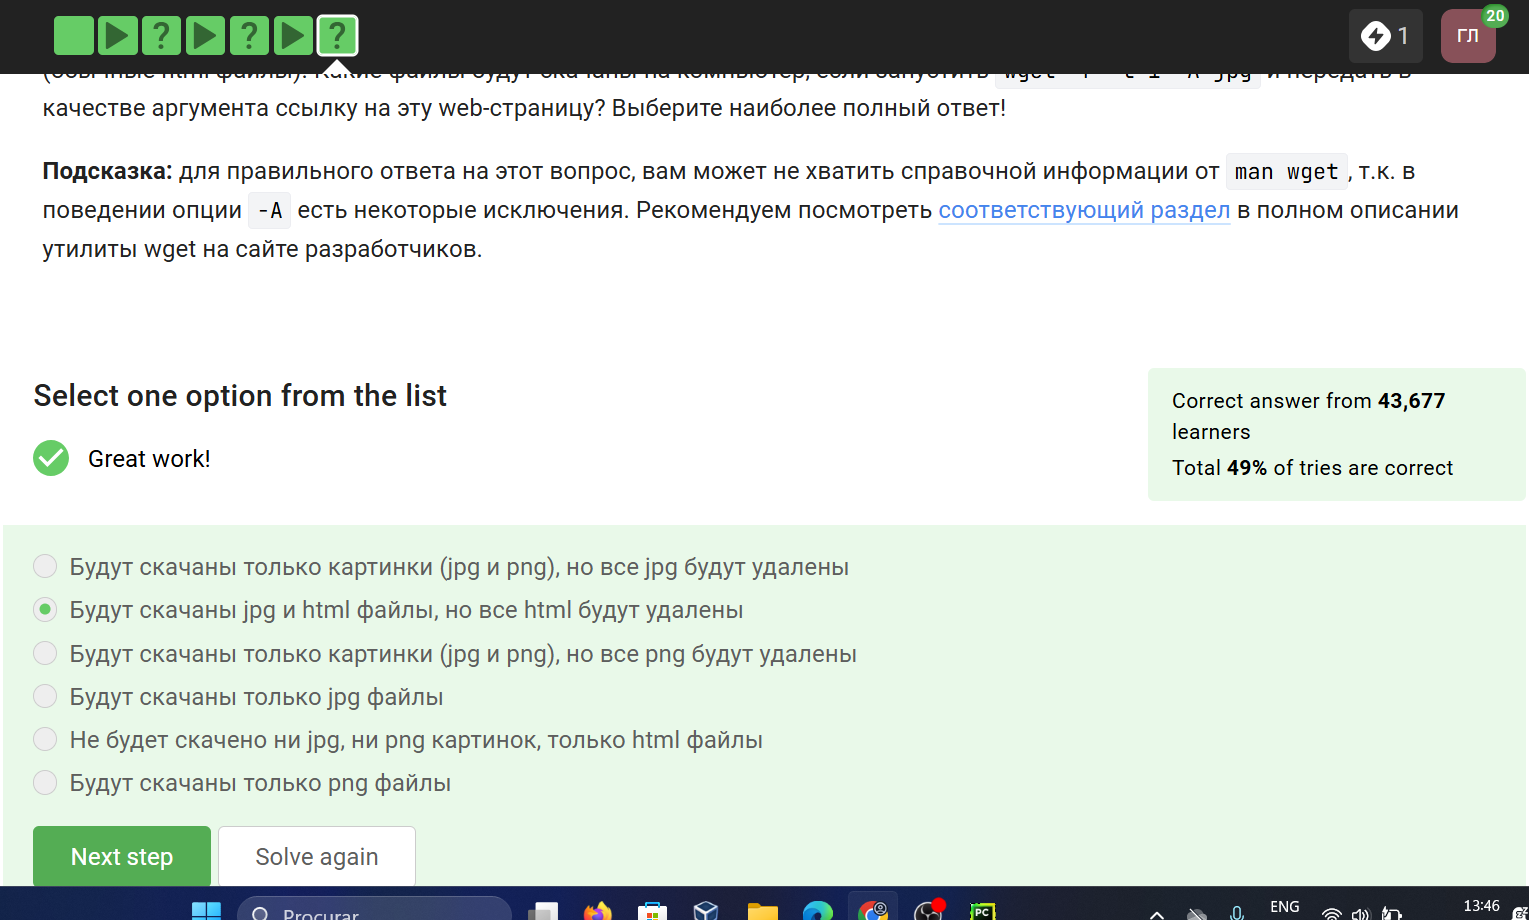
\includegraphics[width=0.7\textwidth,height=\textheight]{image/25.png}
\caption{25}\label{fig:025}
}
\end{figure}

4.2 Типы файлов

Wget предлагает две опции для решения этой проблемы. В описании каждой
опции перечислены краткое имя, длинное имя и эквивалентная команда в
.wgetrc.

`-A acclist' `--accept acclist' `accept = acclist' `--accept-regex
urlregex' `accept-regex = urlregex'

\begin{figure}
\hypertarget{fig:026}{%
\centering
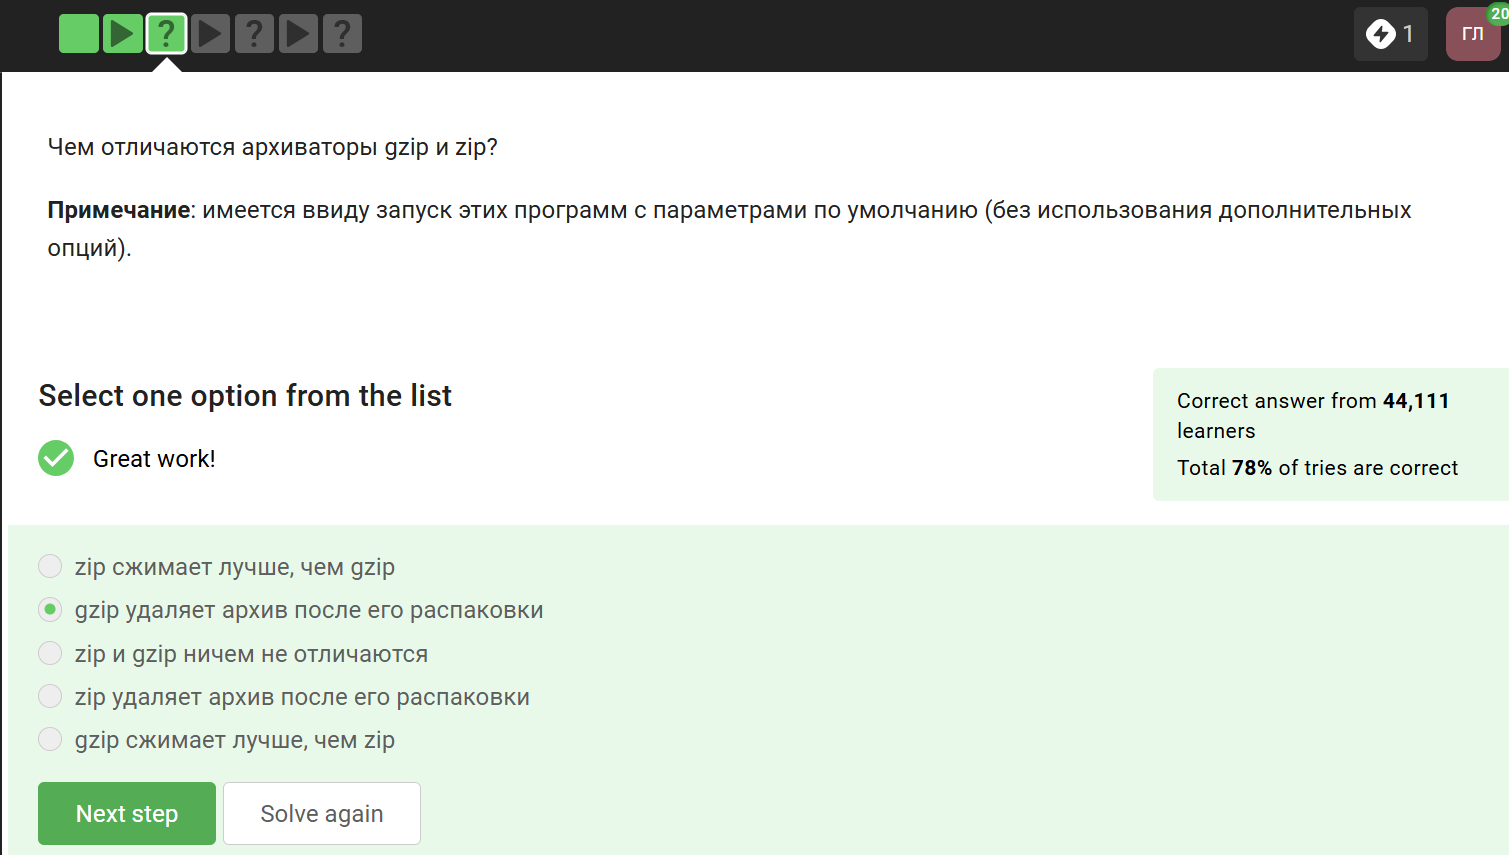
\includegraphics[width=0.7\textwidth,height=\textheight]{image/26.png}
\caption{26}\label{fig:026}
}
\end{figure}

\hypertarget{ux432ux44bux43fux43eux43bux43dux435ux43dux438ux435-ux43bux430ux431ux43eux440ux430ux442ux43eux440ux43dux43eux439-ux440ux430ux431ux43eux442ux44b-18}{%
\section{Выполнение лабораторной
работы}\label{ux432ux44bux43fux43eux43bux43dux435ux43dux438ux435-ux43bux430ux431ux43eux440ux430ux442ux43eux440ux43dux43eux439-ux440ux430ux431ux43eux442ux44b-18}}

\begin{figure}
\hypertarget{fig:027}{%
\centering
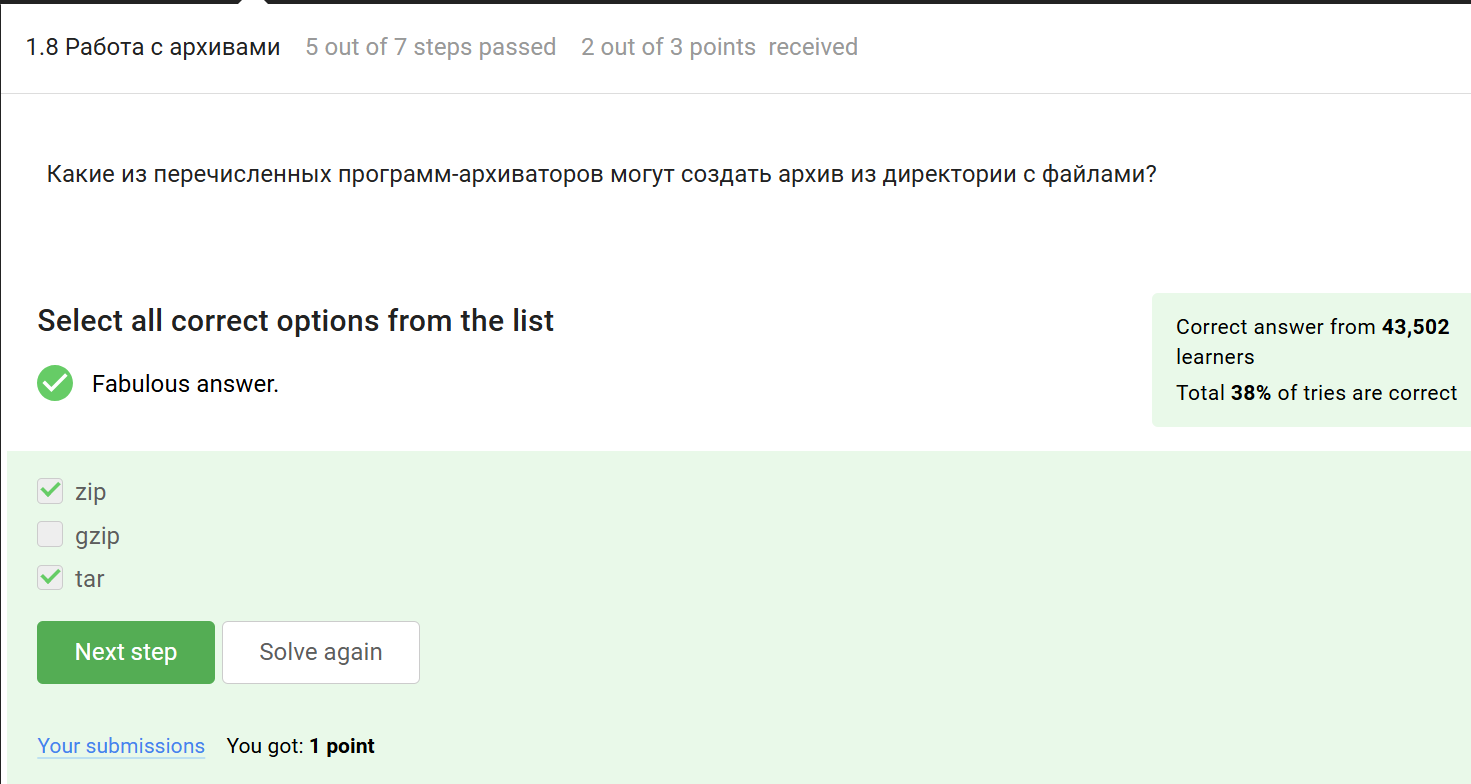
\includegraphics[width=0.7\textwidth,height=\textheight]{image/27.png}
\caption{27}\label{fig:027}
}
\end{figure}

gzip (сокращение от GNU Zip) --- утилита сжатия и восстановления
(декомпрессии) файлов, использующая алгоритм Deflate.

\begin{figure}
\hypertarget{fig:028}{%
\centering
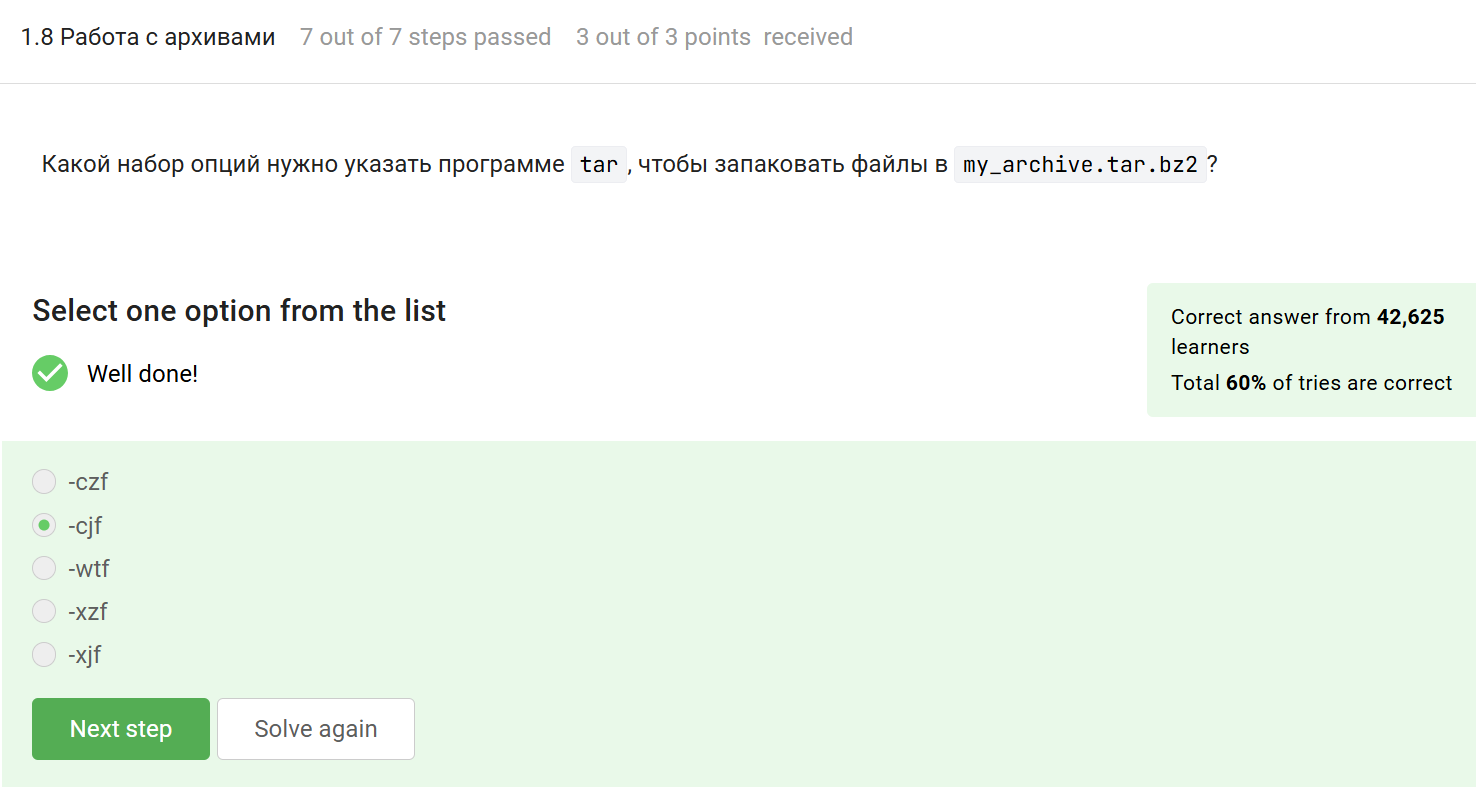
\includegraphics[width=0.7\textwidth,height=\textheight]{image/28.png}
\caption{28}\label{fig:028}
}
\end{figure}

\hypertarget{ux432ux44bux43fux43eux43bux43dux435ux43dux438ux435-ux43bux430ux431ux43eux440ux430ux442ux43eux440ux43dux43eux439-ux440ux430ux431ux43eux442ux44b-19}{%
\section{Выполнение лабораторной
работы}\label{ux432ux44bux43fux43eux43bux43dux435ux43dux438ux435-ux43bux430ux431ux43eux440ux430ux442ux43eux440ux43dux43eux439-ux440ux430ux431ux43eux442ux44b-19}}

c - архиватор

j - указатель на тип архиватора bzip

f - потому что создаем архив в файловой системе

\begin{figure}
\hypertarget{fig:029}{%
\centering
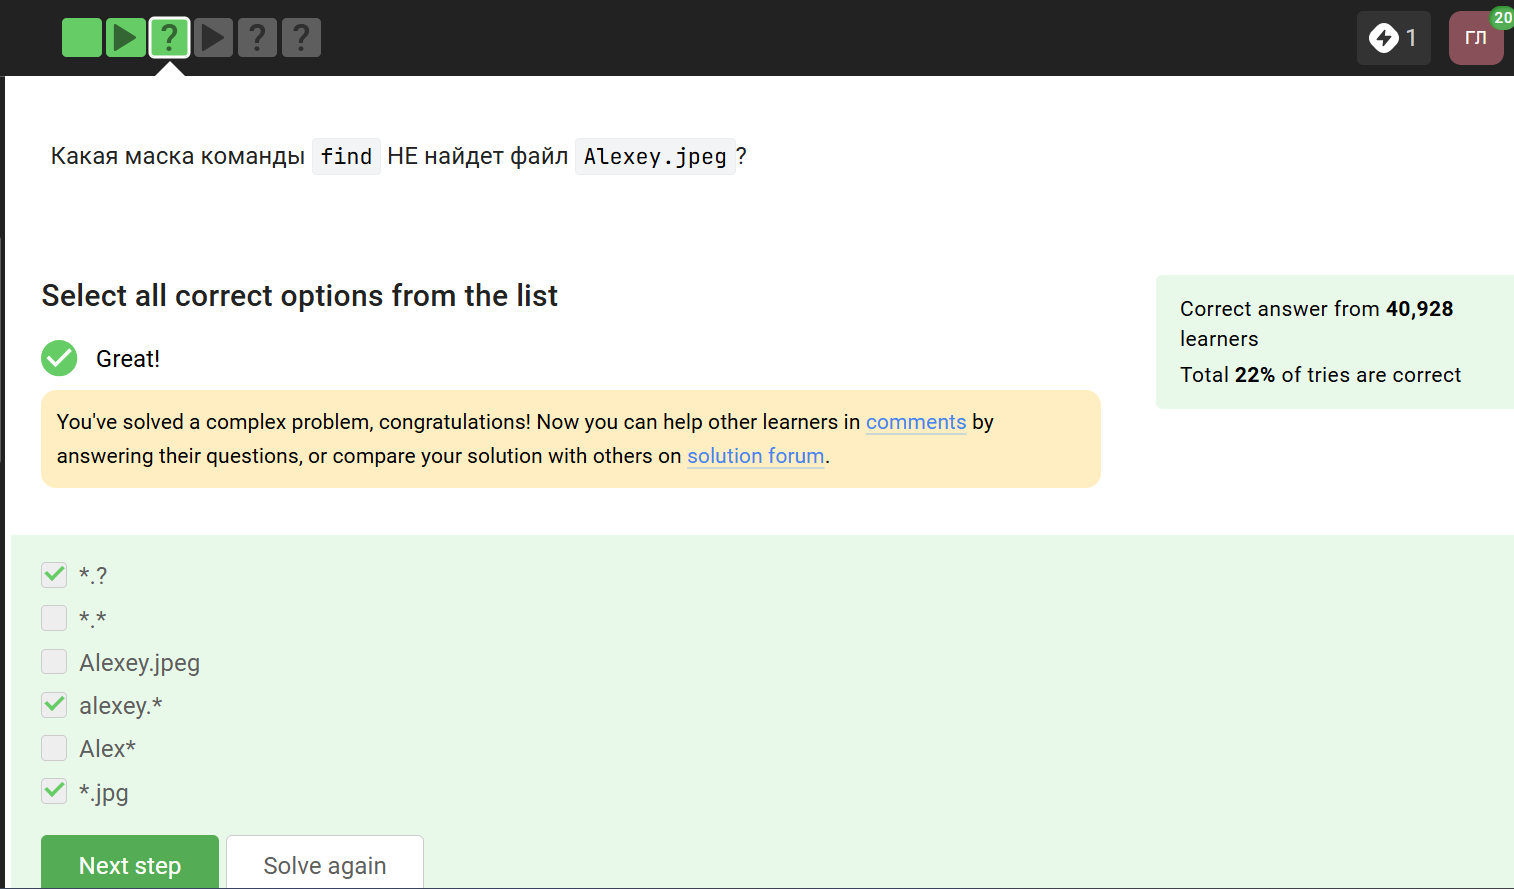
\includegraphics[width=0.7\textwidth,height=\textheight]{image/29.png}
\caption{29}\label{fig:029}
}
\end{figure}

\hypertarget{ux432ux44bux43fux43eux43bux43dux435ux43dux438ux435-ux43bux430ux431ux43eux440ux430ux442ux43eux440ux43dux43eux439-ux440ux430ux431ux43eux442ux44b-20}{%
\section{Выполнение лабораторной
работы}\label{ux432ux44bux43fux43eux43bux43dux435ux43dux438ux435-ux43bux430ux431ux43eux440ux430ux442ux43eux440ux43dux43eux439-ux440ux430ux431ux43eux442ux44b-20}}

\texttt{?} = один символ

\texttt{alexey} = маленькая буква

И файл должен быть \texttt{jpeg}, а не \texttt{jpg}

\begin{figure}
\hypertarget{fig:030}{%
\centering
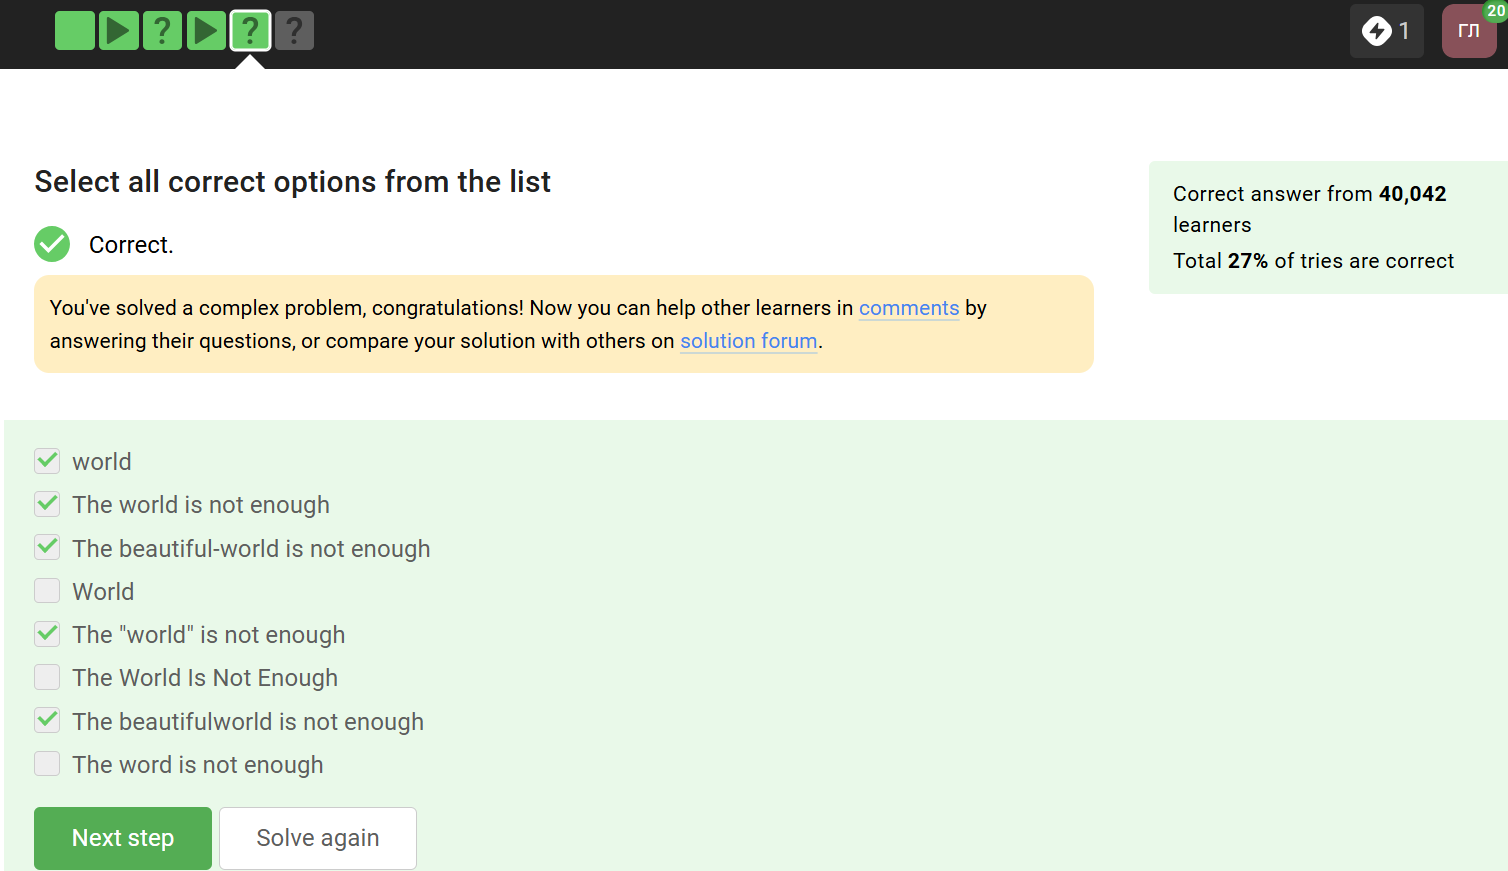
\includegraphics[width=0.7\textwidth,height=\textheight]{image/30.png}
\caption{30}\label{fig:030}
}
\end{figure}

\hypertarget{ux432ux44bux43fux43eux43bux43dux435ux43dux438ux435-ux43bux430ux431ux43eux440ux430ux442ux43eux440ux43dux43eux439-ux440ux430ux431ux43eux442ux44b-21}{%
\section{Выполнение лабораторной
работы}\label{ux432ux44bux43fux43eux43bux43dux435ux43dux438ux435-ux43bux430ux431ux43eux440ux430ux442ux43eux440ux43dux43eux439-ux440ux430ux431ux43eux442ux44b-21}}

Регистр - маленькая буква, слово - \texttt{world}, а не \texttt{word}

\begin{figure}
\hypertarget{fig:031}{%
\centering
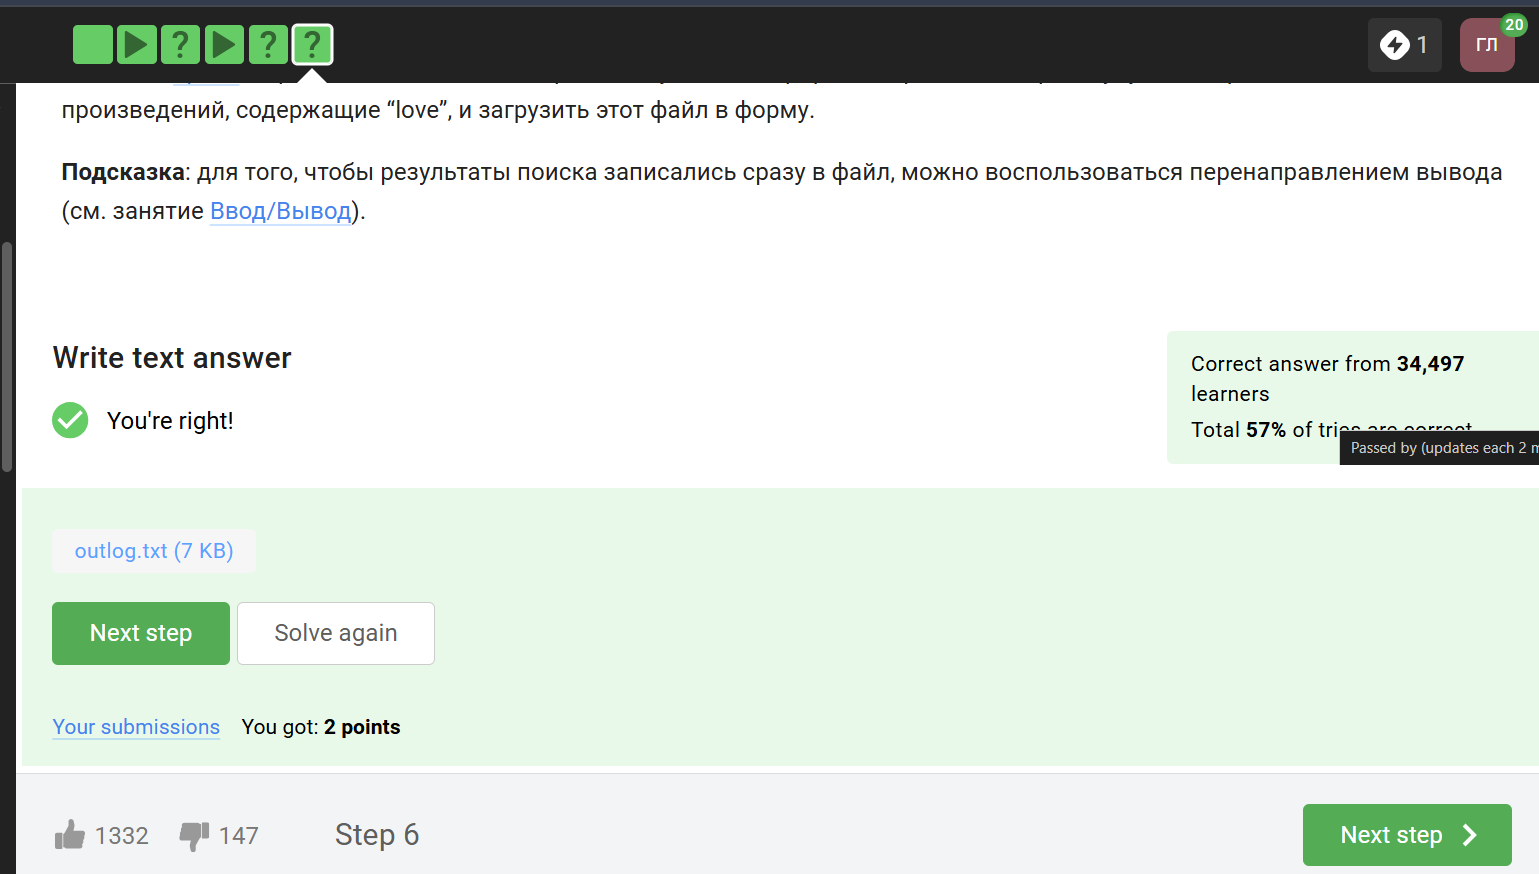
\includegraphics[width=0.7\textwidth,height=\textheight]{image/31.png}
\caption{31}\label{fig:031}
}
\end{figure}

\texttt{grep\ -r\ "love"\ \textasciitilde{}/Shakespeare/\ \textgreater{}\ 1\_m.txt}

\hypertarget{ux432ux44bux432ux43eux434ux44b}{%
\section{Выводы}\label{ux432ux44bux432ux43eux434ux44b}}

Я просмотрела курс и освежила в памяти навыки работы с архивами,
скачивание файлов, команды grep и тп.
